\section{Theoretical Foundations and Empirical Validation}

This section provides the game-theoretic underpinning of the ecosystem designed in \Cref{sec:ecosystem} and empirically validates the framework through a case study.
We first formalize the Bayesian validation game, establish assumptions, and derive incentive compatibility for validators (\S\ref{sec:ic}).
We then characterize threshold-optimal policies for producers (\S\ref{sec:producer_ir}) and consumers (\S\ref{sec:consumer_ir}), prove the existence of a symmetric Bayesian--Nash equilibrium (\S\ref{sec:bne}), and analyze the resulting tokenomics--knowledge dual loop.
Finally, we instantiate the ecosystem as a decentralized question answering system and present simulation results (\S\ref{sec:case_study}).

\subsection{Game-Theoretic Guarantees}
\label{sec:game_theory}

\subsubsection{Model Setup and Assumptions}

We model the ecosystem as a Bayesian game among three types of strategic agents---validators, producers, and consumers---interacting through the mechanism described in \Cref{sec:ecosystem}.

\vspace{1mm}
\noindent\textbf{Game Structure.}
The game proceeds in four stages for each service engagement:
\begin{enumerate}[leftmargin=2em]
    \item \textbf{Nature's move}: Each agent $u \in \mathcal{U}$ is endowed with a private quality type $q_u \in (\frac{1}{2}, 1]$, drawn independently from a common prior distribution $F$ over $(\frac{1}{2}, 1]$. The quality $q_u$ is private information known only to $u$.
    \item \textbf{Validation stage}: The requester (producer or consumer) selects $n$ validators and presents $m$ sample tasks. Each validator $v_i$ chooses an effort level $e_i \in \{0, 1\}$ (shirk or exert effort), then submits a report. Reports are aggregated by majority vote to produce a consensus signal $Z \in \{0, 1\}$.
    \item \textbf{Decision stage}: The requester observes $Z$ and decides whether to proceed (promote or subscribe).
    \item \textbf{Payoff realization}: Tokens are transferred according to the mechanism rules described in \Cref{sec:ecosystem}, and validators' stakes are distributed based on their agreement with the consensus.
\end{enumerate}

\noindent\textbf{Strategy Spaces.}
Each validator's strategy is a mapping from its type $q_v$ to an effort choice $e \in \{0, 1\}$.
Each producer's strategy is a mapping from its type $q_p$ to a promotion decision $d_p \in \{0, 1\}$.
Each consumer's strategy is a mapping from its type and the observed consensus $Z$ to a subscription decision $d_c \in \{0, 1\}$.
A \textit{symmetric} strategy profile requires that all agents of the same role use the same strategy mapping.

\vspace{1mm}
\noindent\textbf{Assumptions.}
We now formalize the assumptions that underpin all subsequent results.

\begin{assumption}[Validator Population and Independence]
\label{assum:validators}
The validation committee consists of $n$ validators (where $n$ is odd to avoid ties), each possessing individual service quality $q_v > \frac{1}{2}$. Validators are drawn independently from the agent population and make decisions independently (no collusion). This independence assumption is operationalized at the protocol level through the \textit{architectural heterogeneity requirement} described in \Cref{sec:ecosystem}, which mandates that validators employ model architectures distinct from the producer and from each other. While architectural diversity cannot eliminate all residual correlation (e.g., from overlapping training corpora), it removes the dominant source of correlated failures---shared model weights and decoding procedures---making approximate independence a defensible modeling choice (see Limitations in \Cref{sec:conclusion} for further discussion).
\end{assumption}

\begin{assumption}[Binary Signal Model]
\label{assum:binary}
For each sample task $x_j$ in the task set, each validator $v_i$ independently produces a per-task binary judgment: $r_{ij} = 1$ (producer's output is correct) or $r_{ij} = 0$ (incorrect). Under truthful effort, $\Pr(r_{ij} = \text{truth}) = q_v$; under shirking (zero effort), $\Pr(r_{ij} = 1) = \frac{1}{2}$ (random guess). Validator $v_i$'s aggregate judgment across the $m$ sample tasks is determined by majority vote over its per-task judgments:
\[
r_i = \mathbbm{1}\!\left[\sum_{j=1}^{m} r_{ij} > \tfrac{m}{2}\right],
\]
so $r_i = 1$ (agree) iff the producer's outputs are correct on a strict majority of sample tasks according to $v_i$'s assessment.
\end{assumption}

\begin{assumption}[Cost Structure]
\label{assum:costs}
Producing a truthful judgment on one task costs $c_u > 0$ (computation, knowledge retrieval). Shirking costs zero. The validation fee satisfies $\tau_{\text{val}} > c_u$ (honest effort is individually viable), and the total validation cost satisfies $mn\tau_{\text{val}} \ll \tau_p \ll \tau_s$ (validation is cheap relative to promotion and subscription).
\end{assumption}

\begin{assumption}[Monotone Likelihood Ratio Property (MLRP)]
\label{assum:mlrp}
The probability that a producer passes majority-vote validation is strictly increasing in its true quality $q_p$. Formally, for the consensus signal $Z \in \{0, 1\}$ (pass/fail), the pass probability $V(q_p) \coloneqq \Pr(Z = 1 \mid q_p)$ is a strictly increasing, continuous function of $q_p$.
\end{assumption}

\begin{remark}[MLRP as a Consequence]
\label{rem:mlrp_derived}
Assumption~\ref{assum:mlrp} is not an independent postulate but follows from Assumptions~\ref{assum:validators}--\ref{assum:costs}: the per-task agreement probability $p_{\text{agree}}(q_p, q_v) = q_p q_v + (1 - q_p)(1 - q_v)$ is strictly increasing in $q_p$ for $q_v > \frac{1}{2}$, and this monotonicity propagates through majority voting to $V(q_p)$. See Appendix~\ref{app:mlrp_derived} for details.
\end{remark}

\noindent\textbf{Extension to $m$ queries.}
Since tasks are i.i.d., the IC condition scales linearly and simplifies to the same per-task condition. We derive all results for $m = 1$ without loss of generality (see Appendix~\ref{app:m_extension}).

\vspace{1mm}
Under these assumptions, we now derive the three layers of incentive guarantees.


\subsubsection{Incentive Compatibility (IC) of Validators}
\label{sec:ic}

The first and most fundamental question is whether the validation mechanism can be trusted at all.
If validators shirk---submitting random judgments to avoid effort costs---then the consensus signal $Z$ carries no information, and the entire ecosystem collapses: producers cannot credibly signal quality, consumers cannot make informed subscription decisions, and the tokenomics--knowledge dual loop breaks down.
We therefore begin by analyzing the validator's decision problem and deriving the conditions under which truthful effort is each validator's strict best response.

Consider a single validator $v_i$ who must choose between exerting truthful effort ($e = 1$) and free-riding ($e = 0$), taking as given that the other $n - 1$ validators play truthfully.
This is a standard Bayesian incentive analysis: we compute the expected payoff under each strategy and identify when truthful effort strictly dominates.

\vspace{1mm}
\noindent\textbf{Payoff Structure.}
Recall from \Cref{sec:ecosystem} that each validator stakes $\sigma$ and receives a reward if its report matches the majority.
We adopt a conservative lower bound on the per-capita reward: if $k$ out of $n$ validators agree with the majority, the total reward pool of $m n \tau_{\text{val}} + n\sigma$ (requester payments plus all stakes) is split among them. In the worst case where all $n$ validators agree, each receives:
\begin{equation}
R_{\min} = \frac{mn\tau_{\text{val}} + n\sigma}{n} = m\tau_{\text{val}} + \sigma.
\end{equation}
For one sample (the per-query case $m = 1$ that we analyze without loss of generality, since tasks are i.i.d.), we have $R_{\min} = \tau_{\text{val}} + \sigma$.
A validator who disagrees with the majority forfeits $\sigma$ and receives nothing.

\vspace{1mm}
\noindent\textbf{Matching Probability under Truthful Play.}
Let $P_{\text{match}}(n, q_v)$ denote the probability that a truthful validator's vote matches the majority when all $n$ validators report truthfully. By conditioning on whether $v_i$'s report is correct (probability $q_v$) or incorrect (probability $1 - q_v$), and computing the probability that a majority of the remaining $n-1$ validators agree in each case, we obtain (see Appendix~\ref{app:pmatch_derivation} for the full derivation):
\begin{equation}
\label{eq:pmatch}
P_{\text{match}}(n, q_v) = q_v \cdot \alpha(n, q_v) + (1 - q_v) \cdot \beta(n, q_v),
\end{equation}
where $\alpha$ and $\beta$ are binomial tail probabilities with parameters $q_v$ and $1-q_v$ respectively.

\begin{proposition}[Properties of $P_{\text{match}}$]
\label{prop:pmatch_properties}
The matching probability satisfies:
\textbf{(i)}~$P_{\text{match}}(n, q_v) > \frac{1}{2}$ for all $q_v > \frac{1}{2}$ (by the Condorcet jury theorem);
\textbf{(ii)}~$P_{\text{match}}$ is strictly increasing in both $q_v$ and $n$;
\textbf{(iii)}~$P_{\text{match}} \to 1$ as $n \to \infty$.
\end{proposition}
\noindent\textit{Proof.} See Appendix~\ref{app:pmatch_properties}. The key insight for (i) is that $P_{\text{match}} \geq q_v^2 + (1-q_v)^2 > \frac{1}{2}$. \qed

\vspace{1mm}
\noindent\textbf{Expected Payoffs.}
Given the payoff structure and matching probability, the expected utilities under the two strategies are:

Under \textbf{truthful effort} ($e = 1$): the validator matches the majority with probability $P_{\text{match}}$, earning $R_{\min}$, and fails to match with probability $1 - P_{\text{match}}$, losing $\sigma$. The effort costs $c_u$:
\begin{equation}
\label{eq:u_truthful}
\mathbb{E}[U \mid e = 1] = P_{\text{match}} \cdot R_{\min} - (1 - P_{\text{match}}) \cdot \sigma - c_u.
\end{equation}

Under \textbf{free-riding} ($e = 0$): the validator submits a random vote, which matches any majority with probability exactly $\frac{1}{2}$ (since a uniform random vote is independent of the majority outcome; see Appendix~\ref{app:freeriding}). Therefore:
\begin{equation}
\label{eq:u_shirk}
\mathbb{E}[U \mid e = 0] = \frac{1}{2} \cdot R_{\min} - \frac{1}{2} \cdot \sigma = \frac{1}{2}(R_{\min} - \sigma).
\end{equation}

\begin{theorem}[IC Condition for Validators]
\label{Strict IC for Validators}
Under Assumptions~\ref{assum:validators}--\ref{assum:costs}, truthful effort is a strict best response for each validator if and only if:
\begin{equation}
\label{eq:ic}
(\tau_{\text{val}} + 2\sigma)\Big(P_{\text{match}}(n, q_v) - \frac{1}{2}\Big) > c_u.
\end{equation}
\end{theorem}

\begin{proof}[Proof sketch (full proof in Appendix~\ref{app:proof_ic})]
Requiring $\mathbb{E}[U \mid e=1] > \mathbb{E}[U \mid e=0]$ and substituting Equations~\eqref{eq:u_truthful}--\eqref{eq:u_shirk}, the algebra reduces to $(R_{\min} + \sigma)(P_{\text{match}} - \frac{1}{2}) > c_u$. The IC condition decomposes into a product of the \textit{total economic stake} $(R_{\min} + \sigma) = \tau_{\text{val}} + 2\sigma$ and the \textit{informational edge} $(P_{\text{match}} - \frac{1}{2})$ that truthful effort provides over random guessing.
\end{proof}

\begin{interpretbox}{Takeaway: Economic Interpretation of Validator IC}
The IC condition $(\tau_{\text{val}} + 2\sigma)(P_{\text{match}} - \frac{1}{2}) > c_u$ decomposes into three interpretable components:
\begin{itemize}[leftmargin=1.5em, itemsep=2pt]
    \item $(\tau_{\text{val}} + 2\sigma)$: \textbf{Total economic exposure}---the validation fee plus twice the stake, capturing the amount ``at risk'' that amplifies the value of being on the right side of consensus.
    \item $(P_{\text{match}} - \frac{1}{2})$: \textbf{Informational advantage}---how much better a truthful vote aligns with the majority compared to a random coin flip. Larger committees and higher-quality validators widen this gap.
    \item $c_u$: \textbf{Effort cost}---the computational expense that must be overcome. IC holds when the marginal benefit of being informed exceeds the cost of becoming informed.
\end{itemize}
\end{interpretbox}

\noindent\textbf{Comparative Statics.}
The IC region---the set of parameters for which~\eqref{eq:ic} holds---expands when:
\begin{enumerate}[leftmargin=2em]
    \item $\tau_{\text{val}}$ or $\sigma$ increases: higher economic exposure amplifies the cost of being wrong.
    \item $q_v$ increases: more capable validators have a larger informational advantage.
    \item $n$ increases: larger committees strengthen the majority, raising $P_{\text{match}}$.
    \item $c_u$ decreases: cheaper effort is easier to incentivize.
\end{enumerate}
In the limit $n \to \infty$, $P_{\text{match}} \to 1$, so IC holds for any finite $c_u$ given sufficient economic exposure. In practice, a moderate committee size $n \in \{5, 9, 17\}$ is sufficient when $q_v$ is reasonably above $\frac{1}{2}$.


\subsubsection{Producer's Threshold-Optimal Promotion}
\label{sec:producer_ir}

Having established that validators can be trusted to report truthfully (Theorem~\ref{Strict IC for Validators}), we now ask the next logical question in the mechanism's causal chain: \textit{given that the consensus signal $Z$ is informative, when should a producer rationally choose to promote its service?}
This is the supply-side participation problem.
If no producer is willing to pay the promotion fee and face validation, the ecosystem has no services to offer---regardless of how well the validation layer works.

The question is non-trivial because promotion involves upfront costs (the promotion fee $\tau_p$ and validation costs $mn\tau_{\text{val}}$) against an uncertain prospect of subscription revenue.

\vspace{1mm}
\noindent\textbf{Setup.}
A producer with true quality $q_p$ considers promoting its service $a_p$. If it proceeds, it pays:
\begin{itemize}
    \item Promotion fee: $\tau_p$
    \item Validation cost: $mn\tau_{\text{val}}$ (paying $n$ validators for $m$ sample tasks)
\end{itemize}
Majority voting among validators generates a public consensus signal $Z \in \{0, 1\}$ (pass/fail). Under Assumption~\ref{assum:mlrp}, the pass probability $V_p(q_p) = \Pr(Z = 1 \mid q_p)$ is strictly increasing in $q_p$.

If the producer passes validation ($Z = 1$) and the consumer subsequently subscribes, the producer receives subscription revenue $\tau_s$ but incurs future service costs $c_s > 0$ (the net present value of all future service obligations). The net surplus from a successful subscription is therefore $\tau_s - c_s$.

\vspace{1mm}
\noindent\textbf{Expected Payoff.}
The producer's expected payoff from promotion is:
\begin{equation}
\label{eq:producer_payoff}
\Pi_p(q_p) = V_p(q_p) \cdot (\tau_s - c_s) - (\tau_p + mn\tau_{\text{val}}).
\end{equation}
The first term is the expected subscription surplus (pass probability times net revenue); the second is the certain upfront cost.

\begin{theorem}[IR-based Policy for Producers]
\label{IR for Producers}
Under Assumption~\ref{assum:mlrp}, there exists a unique quality threshold $\bar{q}_p \in (0, 1)$ such that promotion is the producer's best response if and only if:
\begin{equation}
\label{eq:producer_threshold}
V_p(q_p) \cdot (\tau_s - c_s) \geq \tau_p + mn\tau_{\text{val}} \quad \Longleftrightarrow \quad q_p \geq \bar{q}_p.
\end{equation}
\end{theorem}

\begin{proof}[Proof sketch (full proof in Appendix~\ref{app:proof_producer_ir})]
Since $V_p(q_p) \cdot (\tau_s - c_s)$ is strictly increasing and continuous in $q_p$ (by Assumption~\ref{assum:mlrp}), is negative at $q_p = \frac{1}{2}$ and positive at $q_p = 1$ (by the cost ordering $mn\tau_{\text{val}} \ll \tau_p \ll \tau_s$), the intermediate value theorem yields a unique crossing point $\bar{q}_p$.
\end{proof}

\begin{interpretbox}{Takeaway: Supply-Side Self-Screening}
The threshold $\bar{q}_p$ implements self-screening without centralized curation. Producers below $\bar{q}_p$ know they are likely to fail validation, making promotion unprofitable---they rationally abstain. Producers above $\bar{q}_p$ expect to pass and earn subscription revenue---they rationally promote. The market thus \textit{self-selects} for quality: the very act of paying promotion and validation fees serves as a credible signal of competence, because only agents who expect to pass can afford the risk.
\end{interpretbox}

\noindent\textbf{Comparative Statics.}
The threshold $\bar{q}_p$ responds to mechanism parameters as follows:
\begin{itemize}
    \item Higher $\tau_p$ or $\tau_{\text{val}}$ $\Rightarrow$ higher $\bar{q}_p$: more expensive entry screens more stringently.
    \item Higher $\tau_s$ $\Rightarrow$ lower $\bar{q}_p$: larger subscription revenue attracts more producers.
    \item Larger $m$ or $n$ (more informative validation) $\Rightarrow$ steeper $V_p$ $\Rightarrow$ lower $\bar{q}_p$: better validation allows lower-quality producers to be reliably filtered, so the threshold can be relaxed.
\end{itemize}


\subsubsection{Consumer's Threshold-Optimal Subscription}
\label{sec:consumer_ir}

The analysis so far has established two layers of the mechanism: validators truthfully report (IC), and producers self-screen by promoting only when sufficiently capable (IR). The final piece is the demand side: \textit{given that the consensus $Z$ is informative and that only competent producers enter the market, when should a consumer rationally commit tokens to a subscription?}

This completes the causal chain of the mechanism. The consumer's problem differs from the producer's in a fundamental way: while the producer knows its own quality $q_p$ and decides whether to enter, the consumer does \textit{not} know $q_p$ and must \textit{infer} it from the noisy consensus signal $Z$. This makes the consumer's problem inherently Bayesian---it must form a posterior belief about producer quality and subscribe only when the expected posterior utility justifies the cost.

\vspace{1mm}
\noindent\textbf{Setup.}
The consumer pays subscription fee $\tau_s$ and validation cost $mn\tau_{\text{val}}$ (for the subscription-stage validation). Majority voting produces a consensus signal $Z \in \{0, 1\}$.

Let $V_c(q_p)$ denote the consumer's \textit{per-subscription value function}---the discounted expected utility from delegating future tasks to a producer of quality $q_p$. The only property required for our analysis is that $V_c(\cdot)$ is \textit{strictly increasing and continuous} in $q_p$ (higher producer quality yields higher consumer utility). A concrete parametric form---$V_c(q_p) = \frac{1-\delta^T}{1-\delta}[q_p \cdot b - (1-q_p) \cdot \ell]$ for discount factor $\delta$, horizon $T$, benefit $b > 0$, and loss $\ell \geq 0$---is provided in Appendix~\ref{app:proof_consumer_ir}, but the results hold for any monotone $V_c$.

\vspace{1mm}
\noindent\textbf{Posterior Utility under Validation.}
The consumer does not directly observe $q_p$ but instead observes the consensus signal $Z$.
Using Bayes' rule, the consumer forms a posterior belief over $q_p$ conditional on $Z$:
\begin{equation}
\label{eq:posterior}
f(q_p \mid Z = 1) = \frac{\Pr(Z = 1 \mid q_p) \cdot f(q_p)}{\Pr(Z = 1)} = \frac{V(q_p) \cdot f(q_p)}{\int V(q) f(q) \, dq},
\end{equation}
where $f(\cdot)$ is the prior density over producer quality (from Nature's move).
The posterior expected utility from subscribing, conditional on a ``pass'' signal, is:
\begin{equation}
\label{eq:consumer_posterior}
\mathbb{E}[V_c(q_p) \mid Z = 1] = \int V_c(q_p) \cdot f(q_p \mid Z = 1) \, dq_p.
\end{equation}

Since $V(q_p) = \Pr(Z = 1 \mid q_p)$ is strictly increasing in $q_p$ (Assumption~\ref{assum:mlrp}), the posterior $f(q_p \mid Z = 1)$ assigns higher weight to higher-quality producers compared to the prior. This is the standard Bayesian updating effect: a ``pass'' signal is \textit{good news} about quality.

\vspace{1mm}
\noindent\textbf{Expected Payoff.}
The consumer's expected payoff from subscribing after observing $Z = 1$ is:
\begin{equation}
\label{eq:consumer_payoff}
\Pi_c = \mathbb{E}[V_c(q_p) \mid Z = 1] - (\tau_s + mn\tau_{\text{val}}).
\end{equation}

\begin{theorem}[IR-based Policy for Consumers]
\label{IR-based Policy for Consumers}
Under Assumptions~\ref{assum:mlrp} and the model above, the consumer's optimal subscription policy is a \textit{signal-contingent threshold rule}: subscribe if and only if $Z = 1$ and the posterior expected utility justifies the cost, i.e.,
\begin{equation}
\label{eq:consumer_threshold}
\mathbb{E}[V_c(q_p) \mid Z = 1] \geq \tau_s + mn\tau_{\text{val}}.
\end{equation}
Moreover, this condition is equivalent to an \textit{ex ante quality threshold}: there exists a unique $\bar{q}_c \in (\frac{1}{2}, 1)$ such that the consumer's expected payoff from subscription is non-negative if and only if the producer's true quality satisfies $q_p \geq \bar{q}_c$.
The consumer does not observe $q_p$ directly; rather, the posterior formed via the consensus signal $Z$ implicitly enforces this threshold through Bayesian updating.
\end{theorem}

\begin{proof}[Proof sketch (full proof in Appendix~\ref{app:proof_consumer_ir})]
The posterior expected utility $\mathbb{E}[V_c \mid Z = 1]$ is: (1)~strictly increasing in $q_p$ (by MLRP-induced first-order stochastic dominance of the posterior); (2)~negative at $q_p \to \frac{1}{2}$ and positive at $q_p \to 1$ (by the cost ordering). The intermediate value theorem yields a unique threshold $\bar{q}_c$. The consumer implements this threshold via Bayesian updating on $Z$, without directly observing $q_p$.
\end{proof}

\vspace{1mm}
\noindent\textbf{Interpretation: Demand-Side Disciplined Engagement.}
The threshold $\bar{q}_c$ ensures that consumers do not over-subscribe: they commit tokens only when the posterior evidence of quality (as reflected in the validation consensus) justifies the subscription cost.
This disciplined demand, combined with the producer's supply-side self-screening, creates a \textit{double filter} that concentrates market activity among genuinely capable producers and well-informed consumers.

\noindent\textbf{Interaction with Validator IC.}
The consumer's threshold $\bar{q}_c$ is well-defined \textit{only if} the validation signal $Z$ is informative, which in turn requires that validators exert truthful effort (Theorem~\ref{Strict IC for Validators}).
If validators shirk, $Z$ is uninformative, the posterior collapses to the prior, and no meaningful threshold exists.
The three layers of the mechanism are therefore \textit{interdependent}: validator IC is the foundation upon which both producer IR and consumer IR rest.

\noindent\textbf{Comparative Statics.}
\begin{itemize}
    \item Higher $\tau_s$ or $\tau_{\text{val}}$ $\Rightarrow$ higher $\bar{q}_c$: more expensive subscription demands stronger evidence.
    \item Larger $n$, $m$, or higher $q_v$ (more informative validation) $\Rightarrow$ lower $\bar{q}_c$: better validation enables the consumer to trust the signal at a lower underlying quality.
    \item When a parameter affects both information and cost (e.g., $n$ increases both validation quality and total $\tau_{\text{val}}$ cost), the net effect on $\bar{q}_c$ depends on the specific calibration.
\end{itemize}


\subsubsection{Symmetric BNE and the Tokenomics--Knowledge Dual Loop}
\label{sec:bne}

The preceding three subsections have independently established that each role has a well-defined optimal strategy: validators truthfully report (Theorem~\ref{Strict IC for Validators}), producers self-screen by threshold (Theorem~\ref{IR for Producers}), and consumers subscribe by threshold (Theorem~\ref{IR-based Policy for Consumers}).
However, these results were derived in isolation---each takes the other roles' strategies as given.
The critical remaining question is whether these individually optimal strategies are \textit{mutually consistent}: do they form a stable equilibrium when all three roles play simultaneously?
If not, the ecosystem could unravel despite each individual component being well-designed.

We now show that they are indeed consistent, forming a symmetric Bayesian--Nash equilibrium.

\begin{theorem}[Symmetric Bayesian Nash Equilibrium]
\label{Symmetric Bayesian Nash Equilibrium}
Under Assumptions~\ref{assum:validators}--\ref{assum:mlrp}, if the following three conditions hold simultaneously:
\begin{equation}
\label{eq:bne}
\underbrace{(\tau_{\text{val}} + 2\sigma)\big(P_{\text{match}}(n, q_v) - \tfrac{1}{2}\big) > c_u}_{\text{V-IC: validators truthfully report}},
\quad
\underbrace{q_p \geq \bar{q}_p}_{\text{P-IR: producers self-screen}},
\quad
\underbrace{\mathbb{E}[V_c(q_p) \mid Z = 1] \geq \tau_s + mn\tau_{\text{val}}}_{\text{C-IR: consumers discipline demand}},
\end{equation}
then a symmetric BNE exists in which:
\begin{enumerate}[leftmargin=2em]
    \item Every validator exerts effort and votes truthfully (\S\ref{sec:ic});
    \item Every producer promotes only when its quality exceeds $\bar{q}_p$ (\S\ref{sec:producer_ir});
    \item Every consumer subscribes only when posterior expected utility justifies the cost (\S\ref{sec:consumer_ir}).
\end{enumerate}
Moreover, no agent of any type has incentive to unilaterally deviate from this strategy profile.
\end{theorem}

\begin{proof}[Proof sketch (full proof in Appendix~\ref{app:proof_bne})]
\textit{Non-emptiness:} By Proposition~\ref{prop:pmatch_properties}(i), $P_{\text{match}} > \frac{1}{2}$, so V-IC is satisfiable for appropriate $(\tau_{\text{val}}, \sigma)$. Concretely, $n = 5$, $q_v = 0.8$ gives $P_{\text{match}} \approx 0.942$; setting $\tau_{\text{val}} = \sigma = 1$ yields IC margin $1.326 > c_u$ for any $c_u < 1$. Given V-IC, the IR thresholds $\bar{q}_p, \bar{q}_c$ are well-defined and can be made close to $\frac{1}{2}$ via large $\tau_s$ and informative validation.
\textit{Best responses:} Each role's optimal strategy (Theorems~\ref{Strict IC for Validators}--\ref{IR-based Policy for Consumers}) is derived taking the other roles' strategies as given. Under the proposed profile, each role's assumption about others is satisfied, so all strategies are mutually consistent. Symmetry follows from identical payoff structures within each type.
\end{proof}

\vspace{1mm}
\noindent\textbf{The Tokenomics--Knowledge Dual Loop at Equilibrium.}
At the BNE, all three roles act rationally and consistently, closing the self-reinforcing cycle identified in \Cref{sec:ecosystem}:
\begin{itemize}
    \item Validators produce \textit{credible information} through incentive-compatible effort (IC ensures truthfulness).
    \item Producers \textit{signal competence} through validation-mediated promotion (IR ensures only capable agents enter).
    \item Consumers \textit{reward reliability} through token-backed subscription (IR ensures rational commitment).
\end{itemize}

The resulting token circulation closes the tokenomics--knowledge dual loop introduced in \Cref{sec:ecosystem}: tokens incentivize truthful behavior, which produces reliable information, which in turn sustains token value.

\vspace{1mm}
\noindent\textbf{Dynamic Selection Pressure.}
Beyond static stability, the equilibrium generates evolutionary dynamics across repeated interactions.
Agents with $q_p > \bar{q}_p$ successfully promote, attract subscriptions, and accumulate tokens; agents with $q_p < \bar{q}_p$ fail validation, deplete their reserves, and eventually exit.
This economic selection pressure is empirically validated in \Cref{sec:case_study}.

\begin{interpretbox}{Takeaway: From Individual Rationality to Collective Intelligence}
The symmetric BNE unifies three independently derived conditions---V-IC, P-IR, and C-IR---into a single self-consistent equilibrium. At this equilibrium, no agent of any type can improve its payoff by unilateral deviation: validators truthfully report, producers self-screen for competence, and consumers discipline their demand. The resulting tokenomics--knowledge dual loop is self-reinforcing and generates evolutionary pressure that progressively elevates the ecosystem's aggregate intelligence---without any centralized authority directing the process.
\end{interpretbox}


\subsubsection{Robustness: Relaxing the Idealized Assumptions}
\label{sec:robustness}

The results above rely on Assumptions~\ref{assum:validators}--\ref{assum:mlrp}, which impose idealized conditions: independent validators, identical quality, and zero collusion. We now show that the core results---in particular, the IC condition---are robust to significant relaxations of these assumptions. The key observation is that the entire theoretical chain depends on a single load-bearing property: $P_{\text{match}} > \frac{1}{2}$. Any relaxation that preserves this inequality preserves IC, which in turn preserves IR and the BNE.

\vspace{2mm}
\noindent\textbf{(A) Bounded Sybil Attacks (Relaxing Non-Collusion).}
We replace the non-collusion assumption with a weaker condition: up to $k$ out of $n$ validators may be controlled by a single adversary who coordinates their votes, where $k < \lfloor n/2 \rfloor$. The remaining $h \coloneqq n - k$ validators are honest with quality $q_v > \frac{1}{2}$.

The adversary's optimal strategy is to cast all $k$ votes identically in whichever direction maximizes disruption. Without loss of generality, consider the case where the adversary votes to ``pass'' a low-quality producer. The consensus outcome is then determined by the $h$ honest validators, but with a shifted threshold: ``fail'' requires at least $\lfloor n/2 \rfloor + 1 - 0 = \lfloor n/2 \rfloor + 1$ votes among all $n$, of which $k$ are already cast for ``pass.'' Thus, for the honest majority to override the adversary and produce a ``fail'' verdict, at least $\lfloor n/2 \rfloor + 1$ out of $h + k = n$ total votes must be ``fail,'' meaning at least $\lfloor n/2 \rfloor + 1$ of the $h$ honest validators must vote ``fail.''

For an honest validator $v_i$ voting truthfully, the matching probability under Sybil attack becomes:
\begin{equation}
\label{eq:pmatch_sybil}
P_{\text{match}}^{\text{Sybil}}(n, k, q_v) = \sum_{\theta \in \{0,1\}} \Pr(\theta) \cdot \Pr(v_i \text{ matches majority} \mid \theta, k \text{ adversarial votes}).
\end{equation}
The adversary's votes shift the effective majority threshold for honest validators. However, as long as $h > n/2$---i.e., honest validators hold a strict majority of seats---the honest bloc controls the consensus. The adversary reduces the margin but cannot flip the outcome.

\begin{theorem}[IC under Bounded Sybil Attacks]
\label{thm:sybil_ic}
Let $h = n - k$ denote the number of honest validators, with $k < \lfloor n/2 \rfloor$. If:
\begin{equation}
\label{eq:ic_sybil}
(\tau_{\textup{val}} + 2\sigma)\Big(P_{\textup{match}}^{\textup{Sybil}}(n, k, q_v) - \frac{1}{2}\Big) > c_u,
\end{equation}
then truthful effort remains a strict best response for every honest validator. Moreover, $P_{\textup{match}}^{\textup{Sybil}}(n, k, q_v) > \frac{1}{2}$ holds whenever $h > n/2$ and $q_v > \frac{1}{2}$.
\end{theorem}

\begin{proof}[Proof sketch (full proof in Appendix~\ref{app:proof_sybil})]
The payoff structure and shirking probability ($\frac{1}{2}$) are unchanged from Theorem~\ref{Strict IC for Validators}. The key step is showing $P_{\text{match}}^{\text{Sybil}} > \frac{1}{2}$: when $\theta$ agrees with the adversary, the adversary reinforces truth ($P_{\text{match}}^{\text{Sybil}} \geq P_{\text{match}}$); when $\theta$ opposes, the honest majority ($h > n/2$) overrides via Condorcet. Averaging over both cases preserves $P_{\text{match}}^{\text{Sybil}} > \frac{1}{2}$.
\end{proof}

\noindent\textbf{Interpretation.}
The Sybil attack reduces the honest validators' informational edge $(P_{\text{match}}^{\text{Sybil}} - \frac{1}{2}) < (P_{\text{match}} - \frac{1}{2})$, but the mechanism designer can compensate by increasing the economic stake $(\tau_{\text{val}} + 2\sigma)$. This yields a precise \textit{Sybil resistance budget}: for given $(n, q_v, c_u)$, the maximum tolerable number of adversarial validators is
\begin{equation}
\label{eq:kstar}
k^* = \max\left\{k \in \mathbb{Z}_{\geq 0} : k < \lfloor n/2 \rfloor \;\text{and}\; (\tau_{\text{val}} + 2\sigma)\Big(P_{\text{match}}^{\text{Sybil}}(n, k, q_v) - \tfrac{1}{2}\Big) > c_u\right\}.
\end{equation}
For example, with $n = 9$, $q_v = 0.8$, $\tau_{\text{val}} = \sigma = 1$, and $c_u = 0.5$, the mechanism tolerates up to $k^* = 2$ adversarial validators while maintaining IC for the honest ones. Increasing $\sigma$ (raising the economic cost of attack) directly increases $k^*$.


\vspace{2mm}
\noindent\textbf{(B) Correlated Validators (Relaxing Independence).}
We replace the independence assumption with bounded equicorrelation: for any two honest validators $v_i, v_j$, their per-task errors satisfy $\text{Corr}(r_i, r_j) = \rho \in [0, 1)$. This models residual correlation from overlapping training data that architectural heterogeneity does not fully eliminate.

Under the standard equicorrelated binary model, the joint distribution of validators' reports can be decomposed via a common latent factor: with probability $\rho$, all validators receive an identical (possibly incorrect) signal; with probability $1 - \rho$, they draw independent signals with accuracy $q_v$. This yields:
\begin{equation}
\label{eq:pmatch_corr}
P_{\text{match}}^{\rho}(n, q_v, \rho) = \rho \cdot \bigl[q_v^2 + (1 - q_v)^2\bigr] + (1 - \rho) \cdot P_{\text{match}}(n, q_v).
\end{equation}
The first term corresponds to the correlated regime (all validators receive the same signal, so $v_i$ matches the unanimous majority iff its own signal matches truth, which occurs with probability $q_v^2 + (1-q_v)^2$). The second term is the standard independent case.

Since $q_v^2 + (1 - q_v)^2 > \frac{1}{2}$ for all $q_v \neq \frac{1}{2}$ and $P_{\text{match}}(n, q_v) > \frac{1}{2}$ by Proposition~\ref{prop:pmatch_properties}(i), the convex combination satisfies $P_{\text{match}}^{\rho} > \frac{1}{2}$ for all $\rho \in [0, 1)$ and $q_v > \frac{1}{2}$.

\begin{theorem}[IC under Bounded Correlation]
\label{thm:corr_ic}
For any equicorrelation $\rho \in [0, 1)$ and $q_v > \frac{1}{2}$, the IC condition holds if:
\begin{equation}
\label{eq:ic_corr}
(\tau_{\textup{val}} + 2\sigma)\Big(P_{\textup{match}}^{\rho}(n, q_v, \rho) - \frac{1}{2}\Big) > c_u.
\end{equation}
The maximum tolerable correlation is:
\begin{equation}
\label{eq:rhostar}
\rho^* = 1 - \frac{c_u / (\tau_{\textup{val}} + 2\sigma) - \bigl[q_v^2 + (1-q_v)^2 - \frac{1}{2}\bigr]}{P_{\textup{match}}(n, q_v) - \bigl[q_v^2 + (1-q_v)^2\bigr]},
\end{equation}
provided the denominator is positive (which holds for $n \geq 3$ and $q_v > \frac{1}{2}$).
\end{theorem}

\begin{proof}
From Equation~\eqref{eq:pmatch_corr}, $P_{\text{match}}^{\rho}$ is a linear, strictly decreasing function of $\rho$ (since $P_{\text{match}}(n, q_v) > q_v^2 + (1-q_v)^2$ for $n \geq 3$). Setting $(\tau_{\text{val}} + 2\sigma)(P_{\text{match}}^{\rho} - \frac{1}{2}) = c_u$ and solving for $\rho$ yields the stated $\rho^*$. For $\rho < \rho^*$, IC holds strictly.
\end{proof}

\noindent\textbf{Interpretation.}
Correlation $\rho$ linearly interpolates $P_{\text{match}}$ between the independent-committee value and the single-validator value $q_v^2 + (1-q_v)^2$. Even at high correlation, IC is preserved by raising the economic stake. For example, with $n = 9$, $q_v = 0.8$, $\tau_{\text{val}} = \sigma = 1$, and $c_u = 0.5$, the mechanism tolerates correlation up to $\rho^* \approx 0.72$---a substantial departure from the idealized $\rho = 0$.


\vspace{2mm}
\noindent\textbf{(C) Heterogeneous Validator Quality (Relaxing Identical $q_v$).}
We replace the identical-quality assumption with a heterogeneous population: each validator $v_i$ has quality $q_{v,i} \in (\frac{1}{2}, 1]$, possibly different.

The IC condition for validator $v_i$ becomes type-dependent:
\begin{equation}
\label{eq:ic_hetero}
(\tau_{\text{val}} + 2\sigma)\Big(P_{\text{match},i}(n, \{q_{v,j}\}_{j=1}^n) - \frac{1}{2}\Big) > c_u,
\end{equation}
where $P_{\text{match},i}$ is the probability that $v_i$'s truthful vote matches the majority of the full heterogeneous committee.

A sufficient condition for IC to hold for \textit{all} validators (including the weakest) is:
\begin{equation}
\label{eq:ic_hetero_sufficient}
(\tau_{\text{val}} + 2\sigma)\Big(P_{\text{match}}(n, q_{v,\min}) - \frac{1}{2}\Big) > c_u, \quad \text{where } q_{v,\min} = \min_i q_{v,i}.
\end{equation}
This is conservative: the weakest validator has the lowest $P_{\text{match},i}$, and if IC holds for it, it holds for all stronger validators \textit{a fortiori}. The symmetric BNE generalizes to a \textit{type-dependent BNE} in which each validator's effort decision depends on its own $q_{v,i}$, but the equilibrium structure is preserved: all honest validators exert effort, producers self-screen, and consumers subscribe by threshold.

\vspace{2mm}
\noindent\textbf{Summary of Robustness Results.}
Table~\ref{tab:robustness} summarizes the three relaxations and their impact on the IC condition.

\begin{table}[!htbp]
\centering
\caption{Robustness of IC under relaxed assumptions. In all cases, $P_{\text{match}} > \frac{1}{2}$ is preserved, and increasing the economic stake $(\tau_{\text{val}} + 2\sigma)$ compensates for the reduced informational edge.}
\vspace{2mm}
\setlength{\tabcolsep}{4pt}
\renewcommand{\arraystretch}{1.2}
\small
\begin{tabular}{l|c|c|c}
\toprule
\textbf{Relaxation} & \textbf{Parameter} & \textbf{Condition for IC} & \textbf{Compensation} \\
\midrule
Sybil attack & $k$ adversaries & $k < \lfloor n/2 \rfloor$ & Increase $\sigma$ \\
Correlation & $\rho \in [0, 1)$ & $\rho < \rho^*$ & Increase $n$ or $\sigma$ \\
Heterogeneous $q_v$ & $q_{v,\min}$ & $q_{v,\min} > \frac{1}{2}$ & Increase $\sigma$ \\
\bottomrule
\end{tabular}
\label{tab:robustness}
\end{table}

A unifying insight emerges: the mechanism's robustness is \textit{economically tunable}. Attacks, correlations, and quality heterogeneity all reduce the informational edge $(P_{\text{match}} - \frac{1}{2})$, but the economic stake $(\tau_{\text{val}} + 2\sigma)$ serves as a multiplier that compensates. The mechanism designer can therefore calibrate the stake level to the anticipated adversarial environment, achieving a desired level of robustness without changing the protocol's structure. This is a fundamental advantage of the tokenomics-based design: security is parameterized by economic cost rather than by cryptographic hardness assumptions.


% ===== FIGURES (experiment figures moved from old Methodology) =====

\begin{figure*}[t]
    \centering
    \vspace{-6mm}
    \begin{subfigure}[b]{0.162\linewidth}
        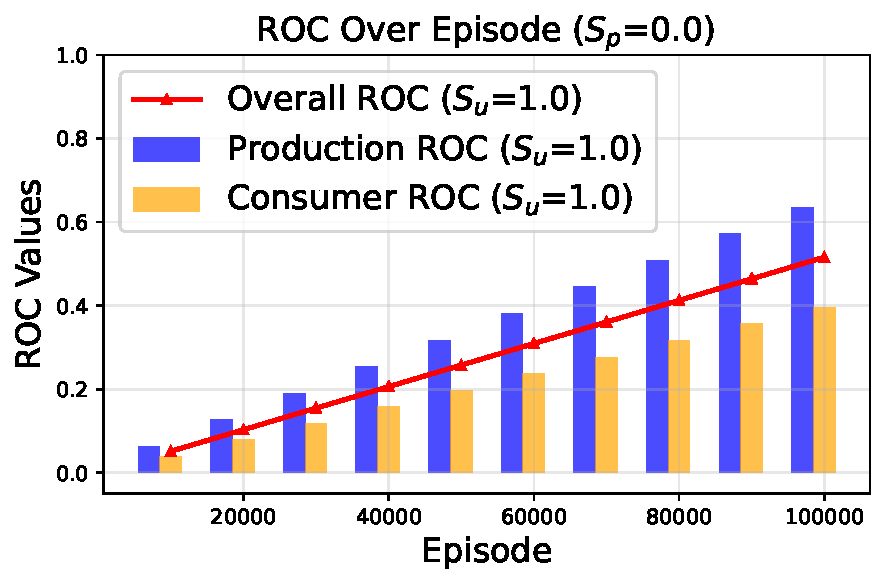
\includegraphics[width=\linewidth]{figures/fixed_sp/population_strategy_0_0_roc.pdf}
    \end{subfigure}
    \begin{subfigure}[b]{0.162\linewidth}
        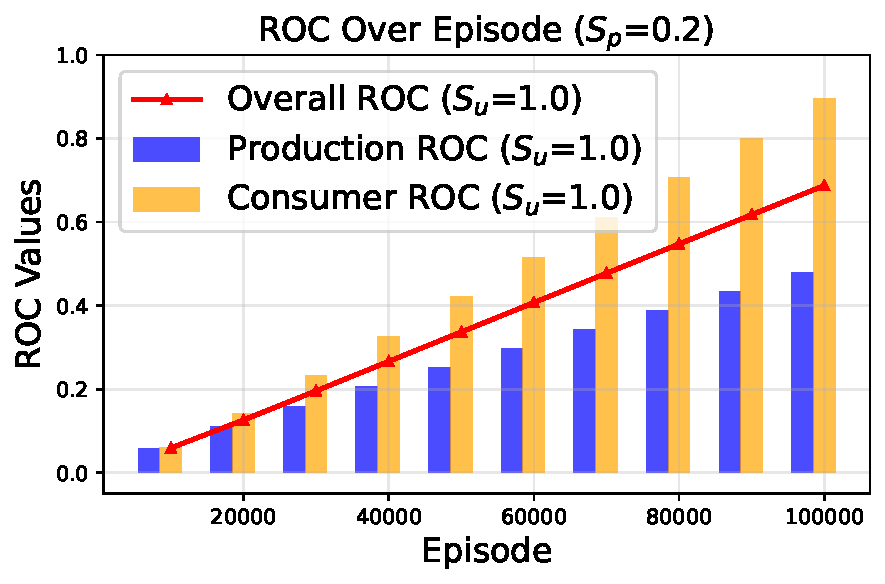
\includegraphics[width=\linewidth]{figures/fixed_sp/population_strategy_0_2_roc.pdf}
    \end{subfigure}
    \begin{subfigure}[b]{0.162\linewidth}
        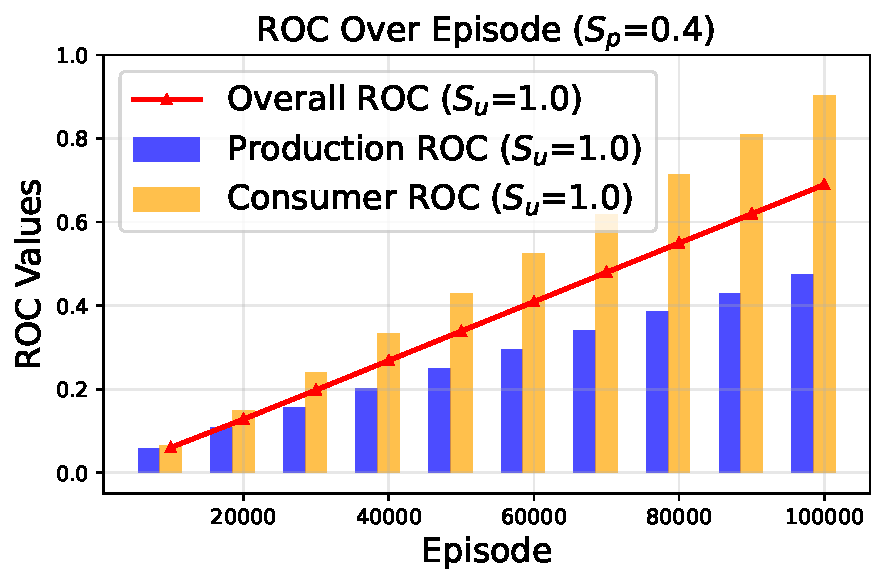
\includegraphics[width=\linewidth]{figures/fixed_sp/population_strategy_0_4_roc.pdf}
    \end{subfigure}
    \begin{subfigure}[b]{0.162\linewidth}
        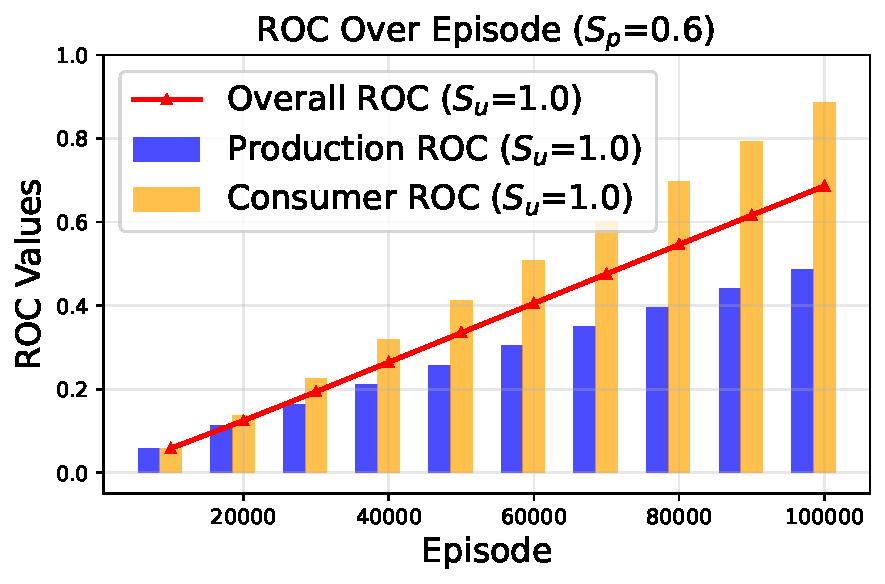
\includegraphics[width=\linewidth]{figures/fixed_sp/population_strategy_0_6_roc.pdf}
    \end{subfigure}
    \begin{subfigure}[b]{0.162\linewidth}
        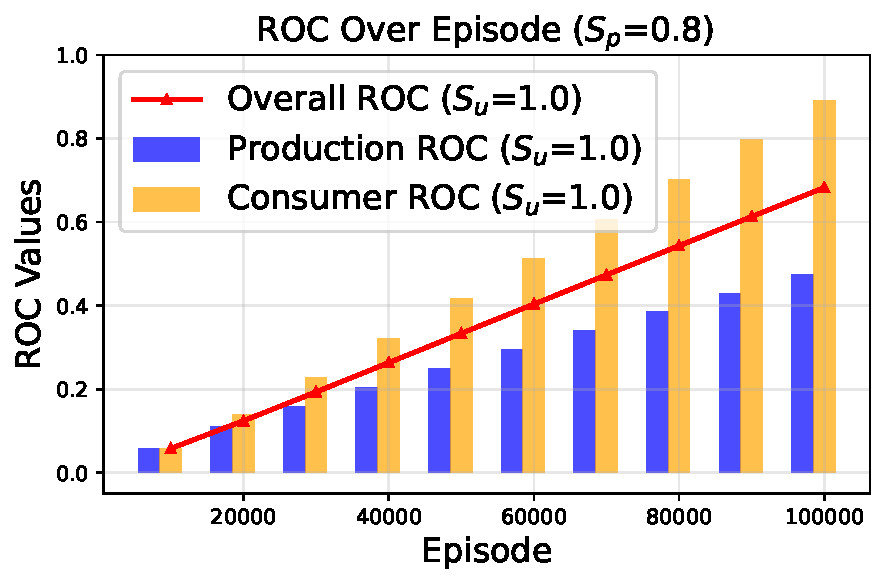
\includegraphics[width=\linewidth]{figures/fixed_sp/population_strategy_0_8_roc.pdf}
    \end{subfigure}
    \begin{subfigure}[b]{0.162\linewidth}
        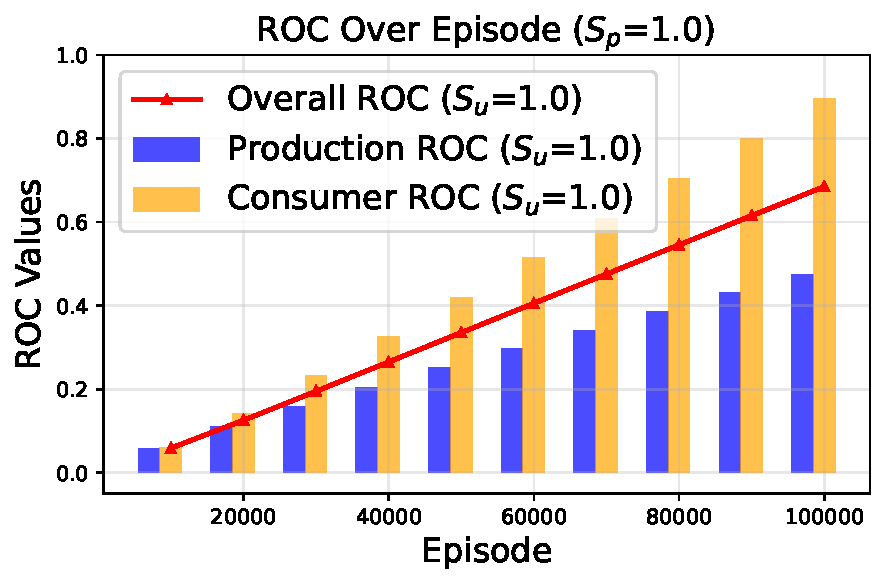
\includegraphics[width=\linewidth]{figures/fixed_sp/population_strategy_1_0_roc.pdf}
    \end{subfigure}
    \vspace{1mm}
    \begin{subfigure}[b]{0.162\linewidth}
        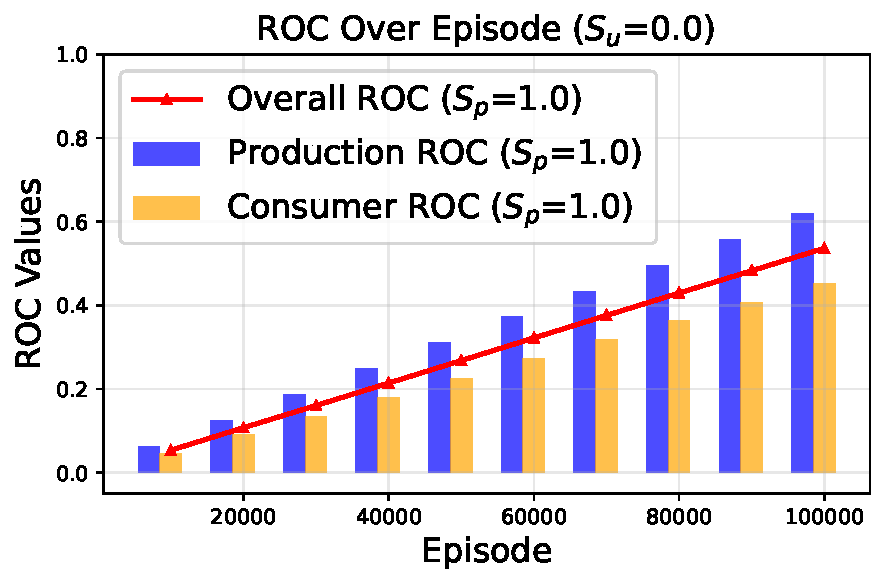
\includegraphics[width=\linewidth]{figures/fixed_su/user_strategy_0_0_roc.pdf}
    \end{subfigure}
    \begin{subfigure}[b]{0.162\linewidth}
        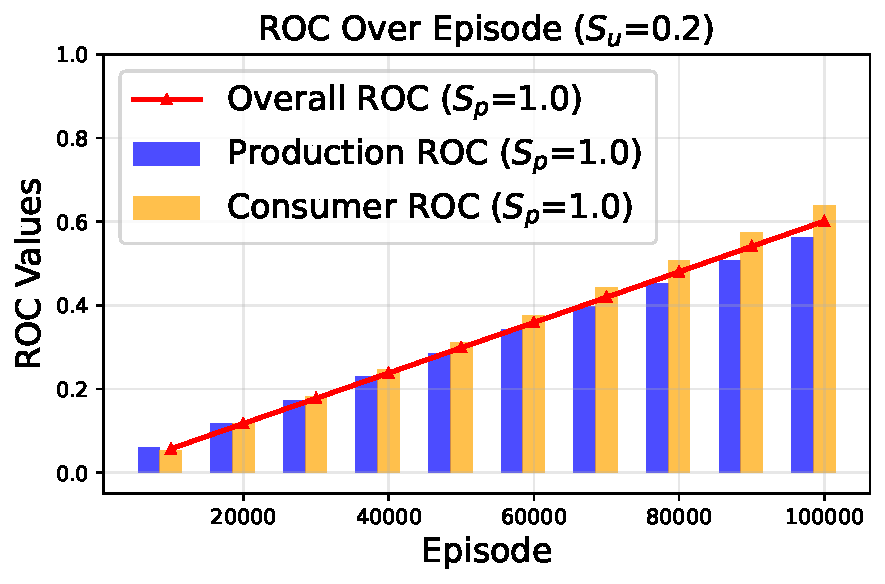
\includegraphics[width=\linewidth]{figures/fixed_su/user_strategy_0_2_roc.pdf}
    \end{subfigure}
    \begin{subfigure}[b]{0.162\linewidth}
        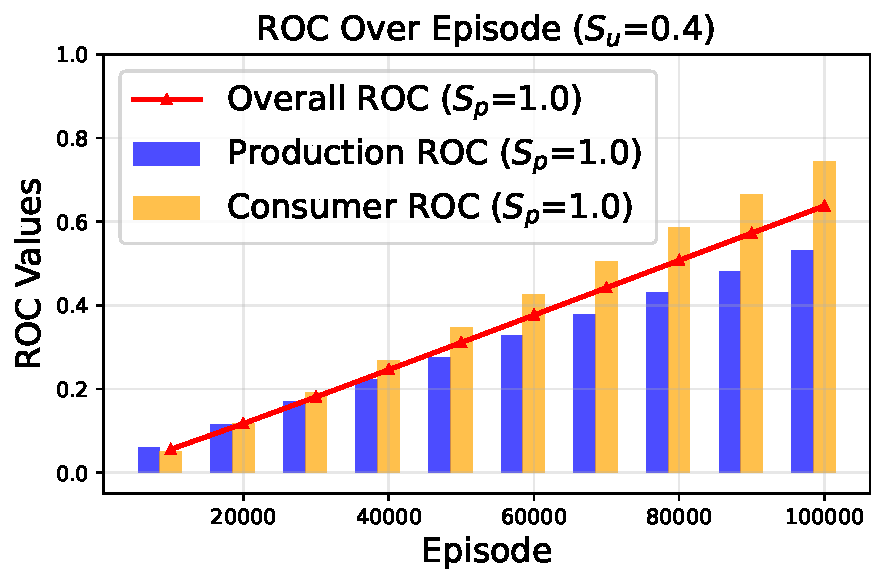
\includegraphics[width=\linewidth]{figures/fixed_su/user_strategy_0_4_roc.pdf}
    \end{subfigure}
    \begin{subfigure}[b]{0.162\linewidth}
        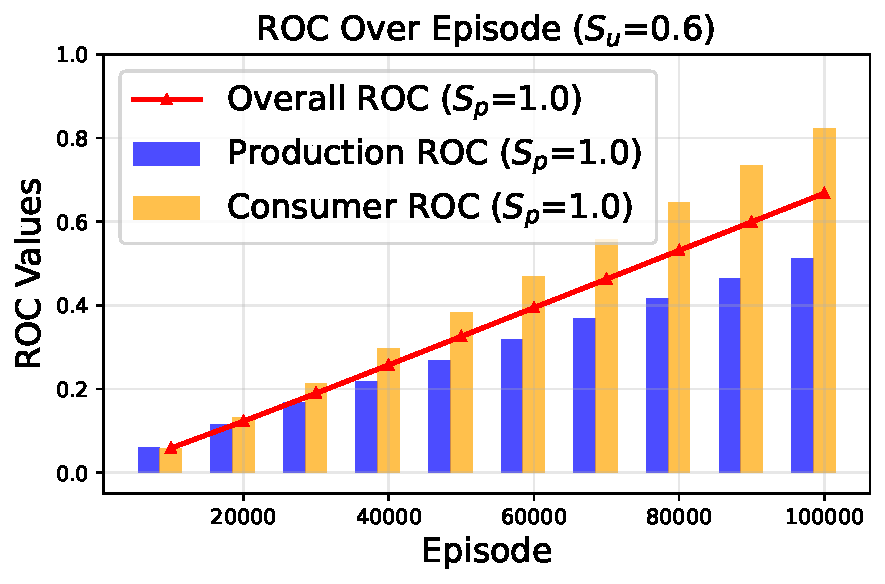
\includegraphics[width=\linewidth]{figures/fixed_su/user_strategy_0_6_roc.pdf}
    \end{subfigure}
    \begin{subfigure}[b]{0.162\linewidth}
        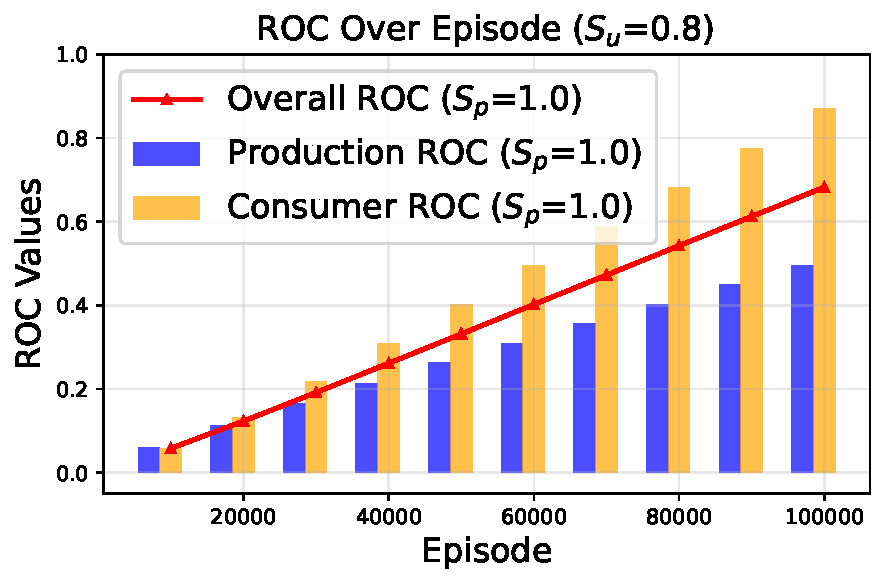
\includegraphics[width=\linewidth]{figures/fixed_su/user_strategy_0_8_roc.pdf}
    \end{subfigure}
    \begin{subfigure}[b]{0.162\linewidth}
        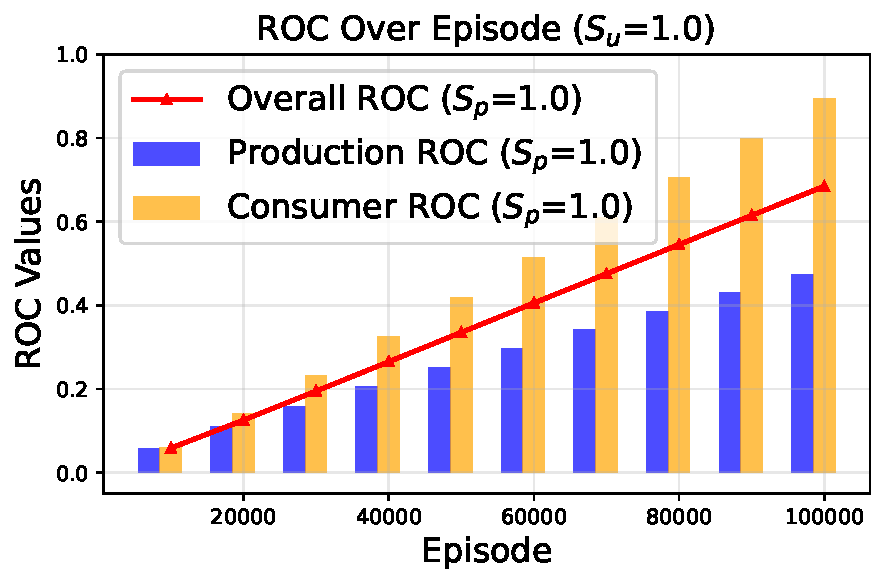
\includegraphics[width=\linewidth]{figures/fixed_su/user_strategy_1_0_roc.pdf}
    \end{subfigure}
    \vspace{-4mm}
    \caption{ROC comparison over 100,000 episodes under different strategy configurations. Top row: varying $S_p$ (proportion of rational agents) with $S_u = 1$. Bottom row: varying $S_u$ (strategy update probability) with $S_p = 1$.}
    \label{fig:roc_comp}
    \vspace{-1mm}
\end{figure*}

\begin{figure*}[t]
    \centering
    \begin{subfigure}[b]{0.162\linewidth}
        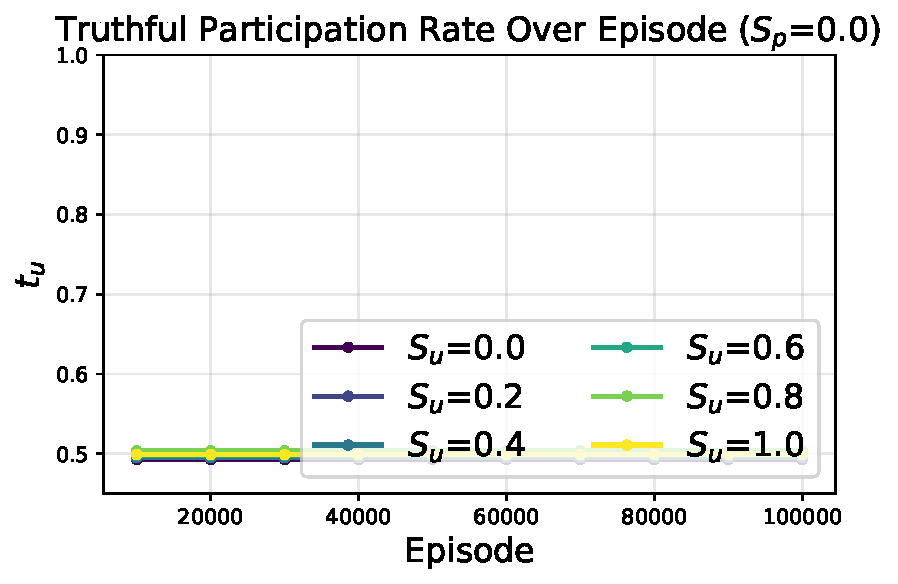
\includegraphics[width=\linewidth]{figures/fixed_sp/population_strategy_0_0_hard.pdf}
    \end{subfigure}
    \begin{subfigure}[b]{0.162\linewidth}
        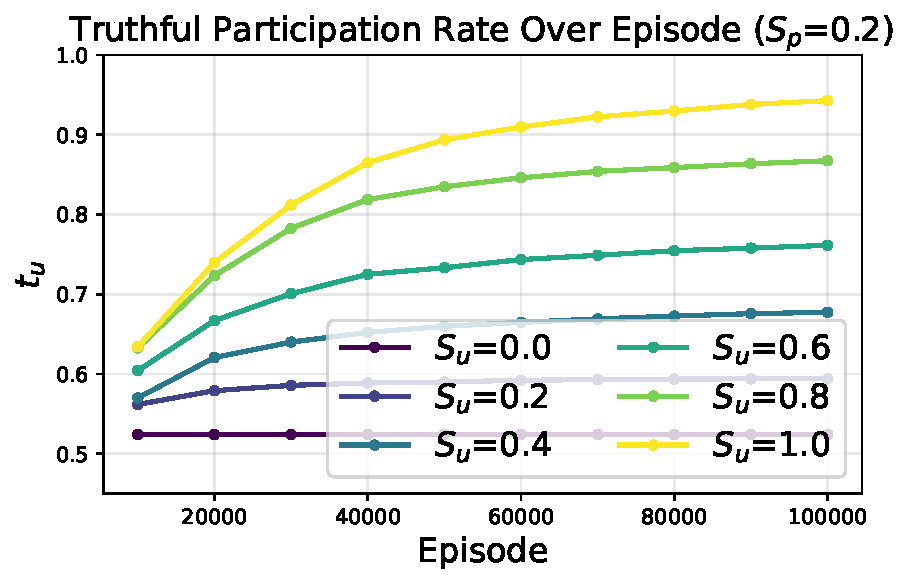
\includegraphics[width=\linewidth]{figures/fixed_sp/population_strategy_0_2_hard.pdf}
    \end{subfigure}
    \begin{subfigure}[b]{0.162\linewidth}
        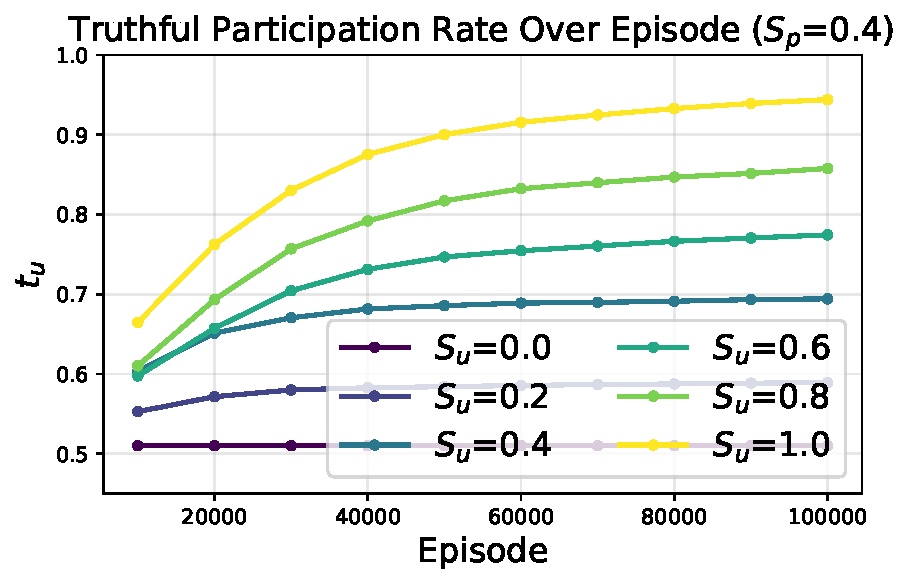
\includegraphics[width=\linewidth]{figures/fixed_sp/population_strategy_0_4_hard.pdf}
    \end{subfigure}
    \begin{subfigure}[b]{0.162\linewidth}
        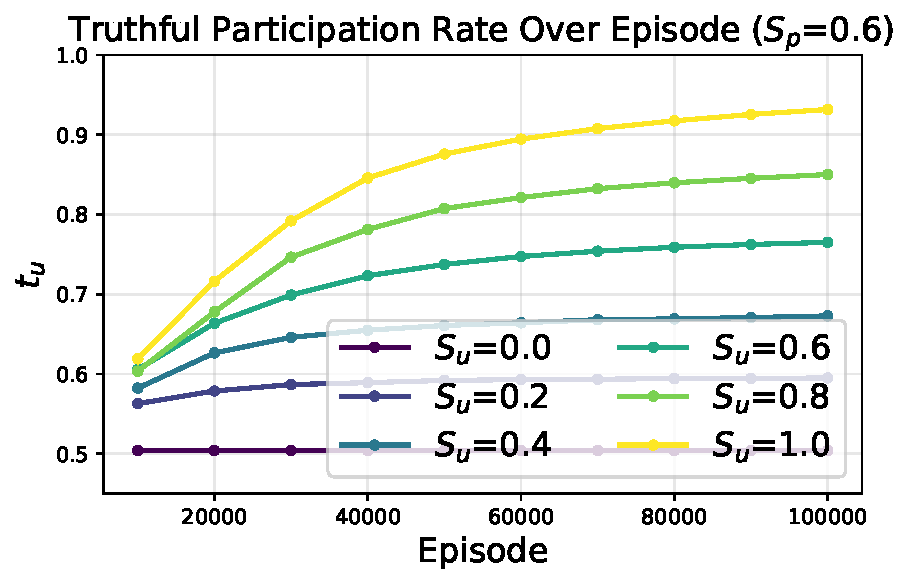
\includegraphics[width=\linewidth]{figures/fixed_sp/population_strategy_0_6_hard.pdf}
    \end{subfigure}
    \begin{subfigure}[b]{0.162\linewidth}
        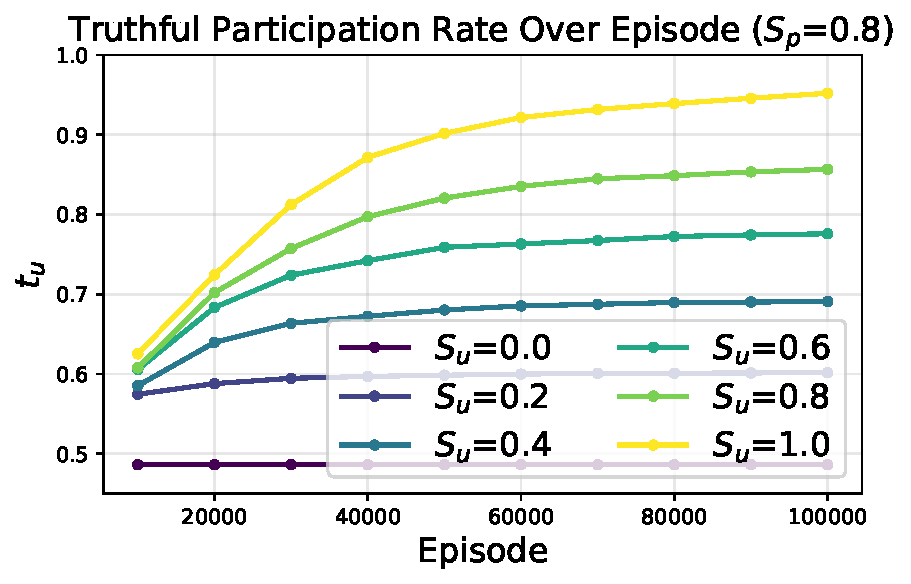
\includegraphics[width=\linewidth]{figures/fixed_sp/population_strategy_0_8_hard.pdf}
    \end{subfigure}
    \begin{subfigure}[b]{0.162\linewidth}
        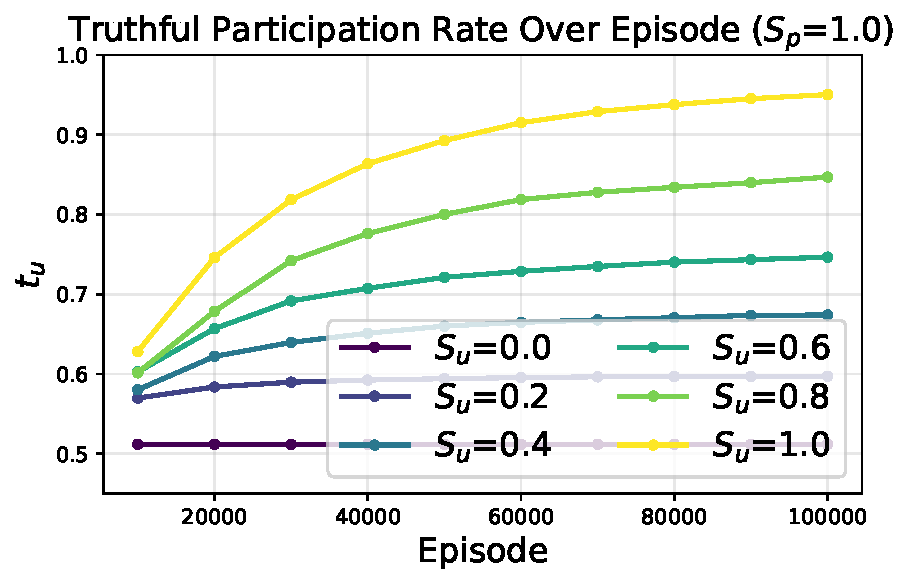
\includegraphics[width=\linewidth]{figures/fixed_sp/population_strategy_1_0_hard.pdf}
    \end{subfigure}
    \vspace{1mm}
    \begin{subfigure}[b]{0.162\linewidth}
        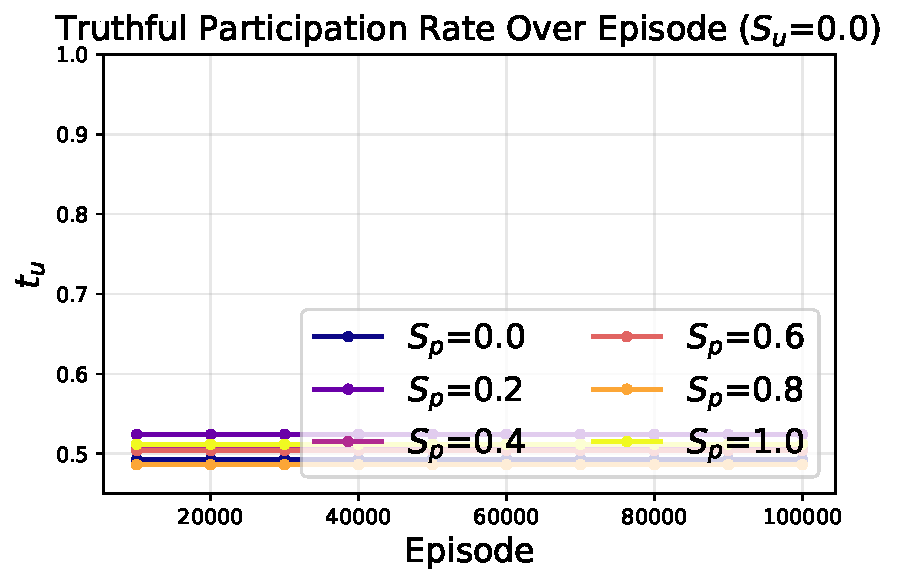
\includegraphics[width=\linewidth]{figures/fixed_su/user_strategy_0_0_hard.pdf}
    \end{subfigure}
    \begin{subfigure}[b]{0.162\linewidth}
        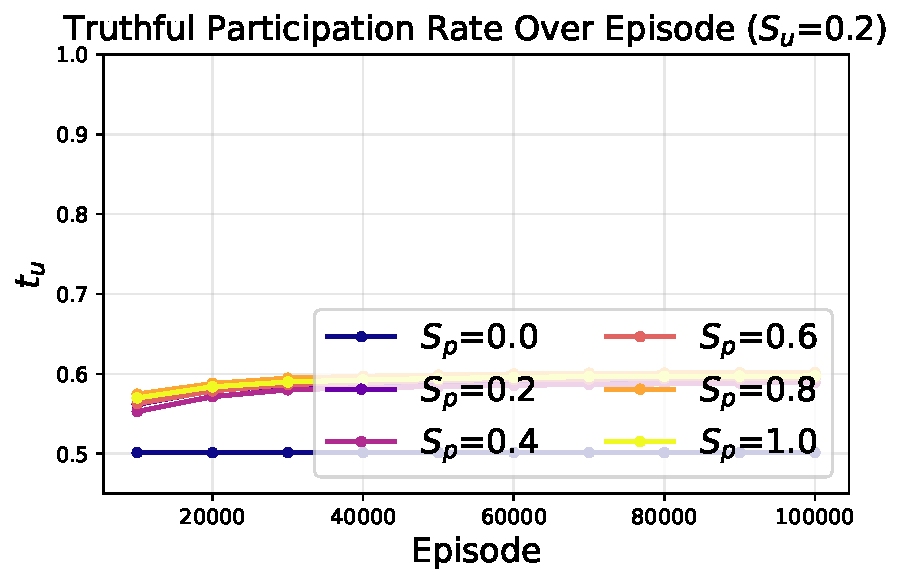
\includegraphics[width=\linewidth]{figures/fixed_su/user_strategy_0_2_hard.pdf}
    \end{subfigure}
    \begin{subfigure}[b]{0.162\linewidth}
        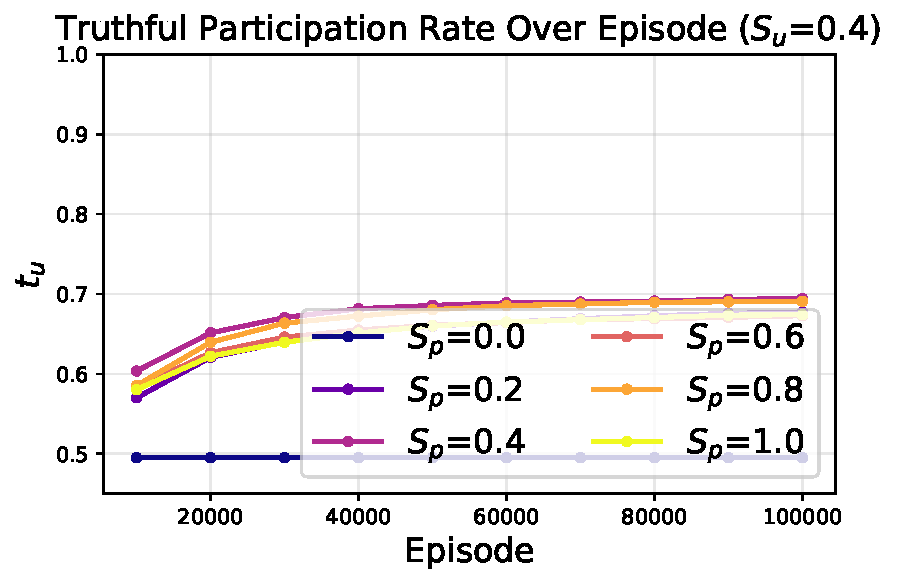
\includegraphics[width=\linewidth]{figures/fixed_su/user_strategy_0_4_hard.pdf}
    \end{subfigure}
    \begin{subfigure}[b]{0.162\linewidth}
        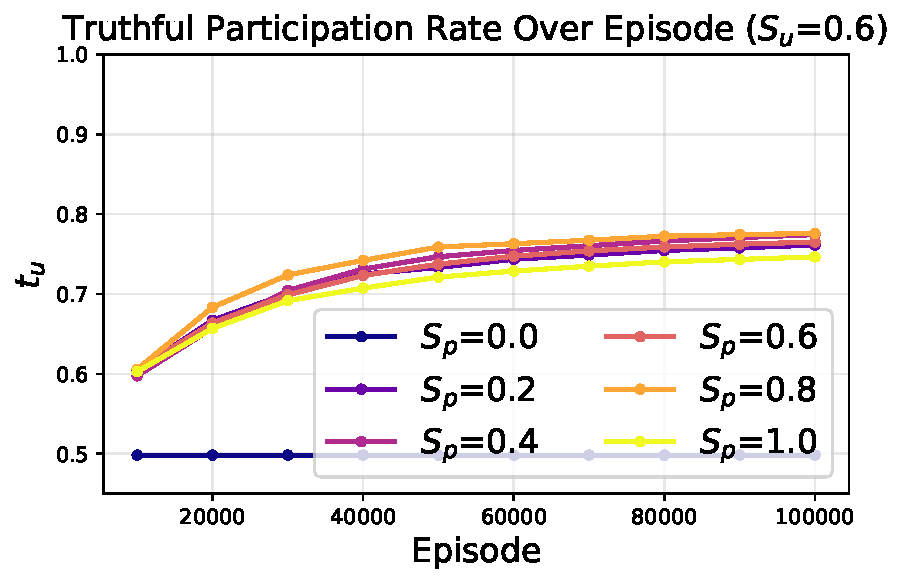
\includegraphics[width=\linewidth]{figures/fixed_su/user_strategy_0_6_hard.pdf}
    \end{subfigure}
    \begin{subfigure}[b]{0.162\linewidth}
        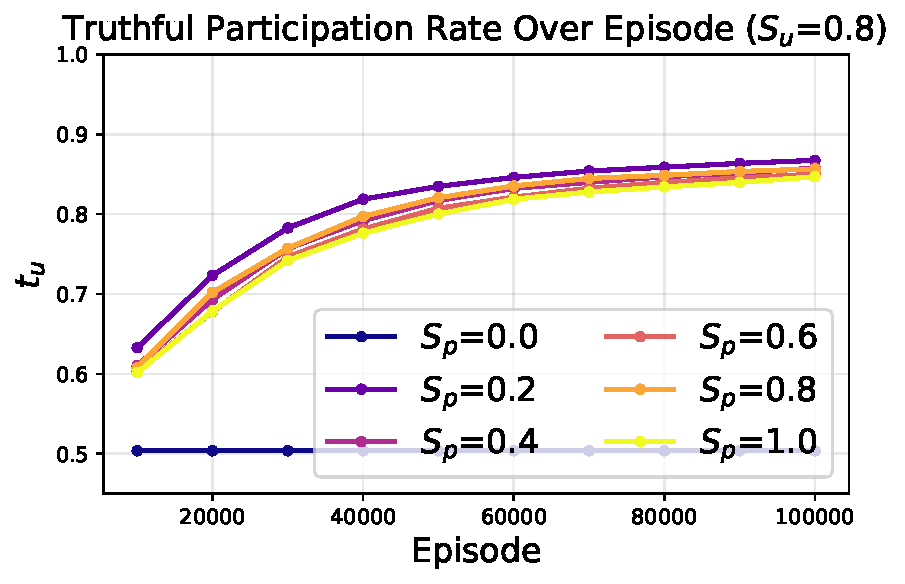
\includegraphics[width=\linewidth]{figures/fixed_su/user_strategy_0_8_hard.pdf}
    \end{subfigure}
    \begin{subfigure}[b]{0.162\linewidth}
        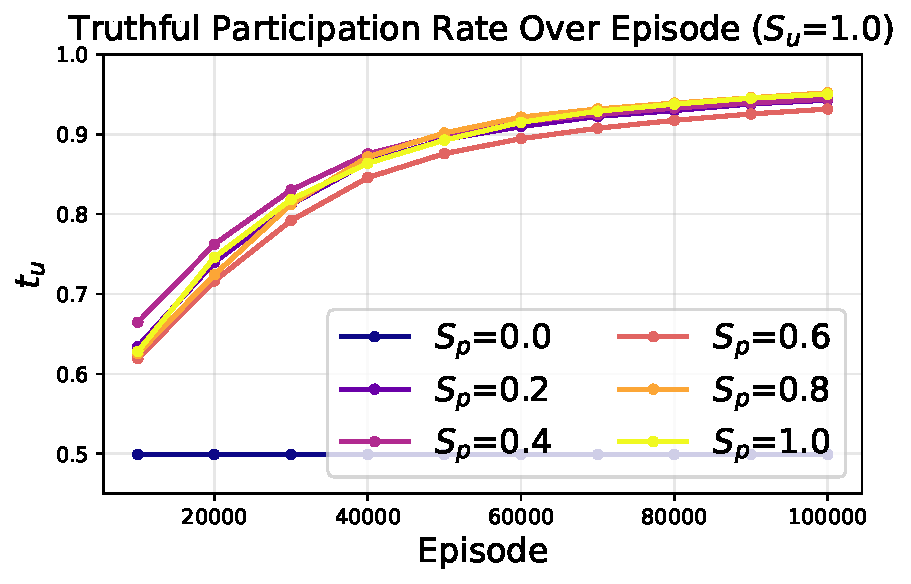
\includegraphics[width=\linewidth]{figures/fixed_su/user_strategy_1_0_hard.pdf}
    \end{subfigure}
    \vspace{-3mm}
    \caption{Truthful participation rate comparison under different $S_u$ and $S_p$ configurations. As rational agents increase ($S_p \uparrow$) and update their strategies more frequently ($S_u \uparrow$), the population converges toward higher truthful participation.}
    \label{fig:truthful_participation}
\end{figure*}


% =========================================================================
\subsection{Case Study: Decentralized Question Answering (DeQA)}
\label{sec:case_study}
% =========================================================================

The theoretical analysis above establishes that the ecosystem admits a self-enforcing equilibrium under appropriate parameter conditions.
We now ask: \textit{do these predictions hold in practice?}
Specifically, we seek to verify three empirical implications of the theory:
(i) that rational agents converge toward truthful strategies under the tokenomics--knowledge dual loop (predicted by the IC and IR conditions);
(ii) that the validation mechanism improves welfare, with performance depending on committee size $n$ (predicted by the comparative statics of Theorem~\ref{Strict IC for Validators});
and (iii) that the mechanism amplifies genuine quality but cannot compensate for fundamentally unreliable agents (predicted by the MLRP-based threshold structure of Theorems~\ref{IR for Producers}--\ref{IR-based Policy for Consumers}).

To test these predictions, we instantiate the ecosystem as a \textbf{De}centralized \textbf{Q}uestion \textbf{A}nswering system (\textbf{DeQA}).
Question answering serves as a natural testbed: consumer agents issue domain-specific queries, producer agents provide answers drawing on their knowledge bases, and validator agents independently generate answers and compare them against the producer's output to assess service alignment.
While we use QA for concreteness, we emphasize that the mechanism design, theoretical results, and incentive structures are domain-agnostic and apply to any knowledge-intensive agent collaboration scenario (e.g., code generation, data analysis, research synthesis).

These empirical implications motivate three research questions:

$\bullet$~\textbf{RQ1} (Rationality and Evolution): How do agent strategies influence ecosystem evolution?

$\bullet$~\textbf{RQ2} (Validation Mechanism): How does the number of validators affect net welfare?

$\bullet$~\textbf{RQ3} (Service Quality): What is the relationship between service quality and overall welfare?


\begin{figure*}[t]
    \centering
    \vspace{-6mm}
    \begin{subfigure}[b]{0.195\linewidth}
        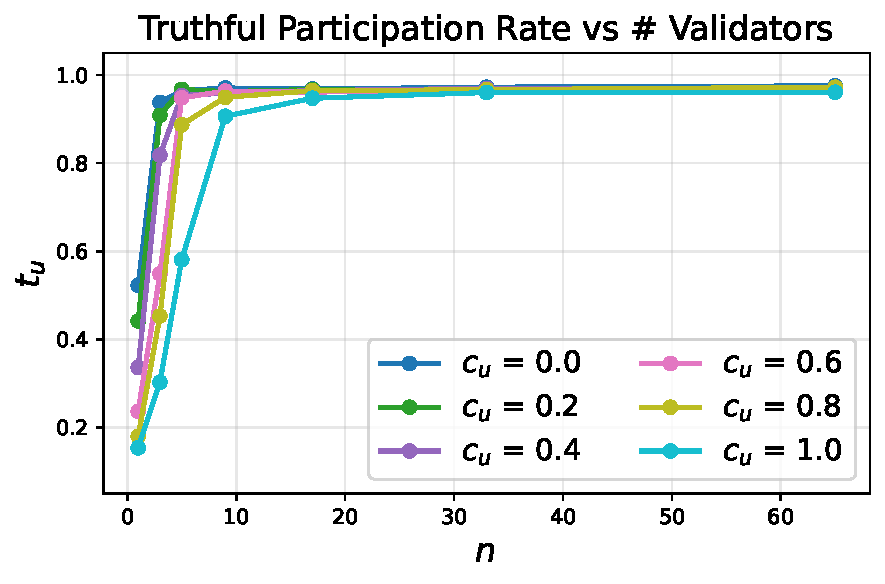
\includegraphics[width=\linewidth]{figures/hard/hard_all_costs.pdf}
        \caption{Truthful Participation}
    \end{subfigure}
    \hfill
    \begin{subfigure}[b]{0.195\linewidth}
        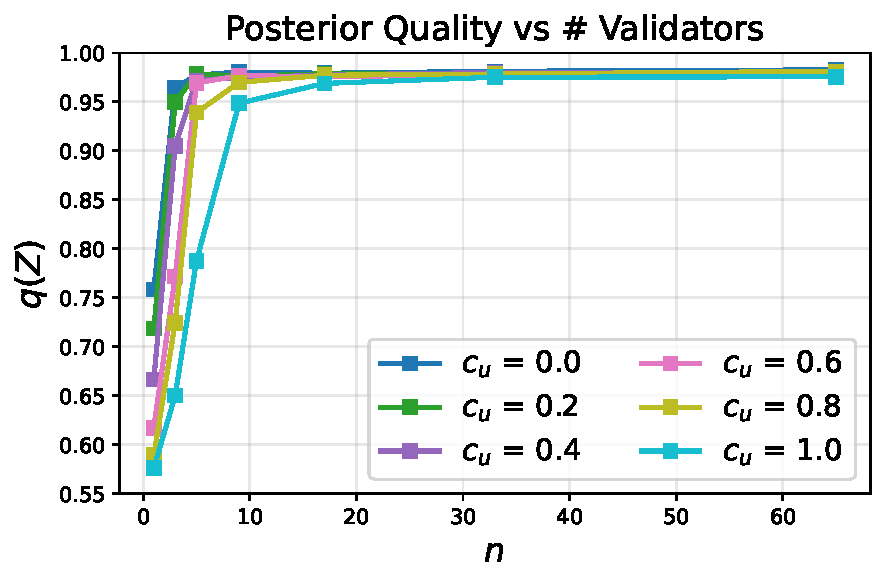
\includegraphics[width=\linewidth]{figures/hard/weighted_p_all_costs.pdf}
        \caption{Posterior Quality}
    \end{subfigure}
    \hfill
    \begin{subfigure}[b]{0.195\linewidth}
        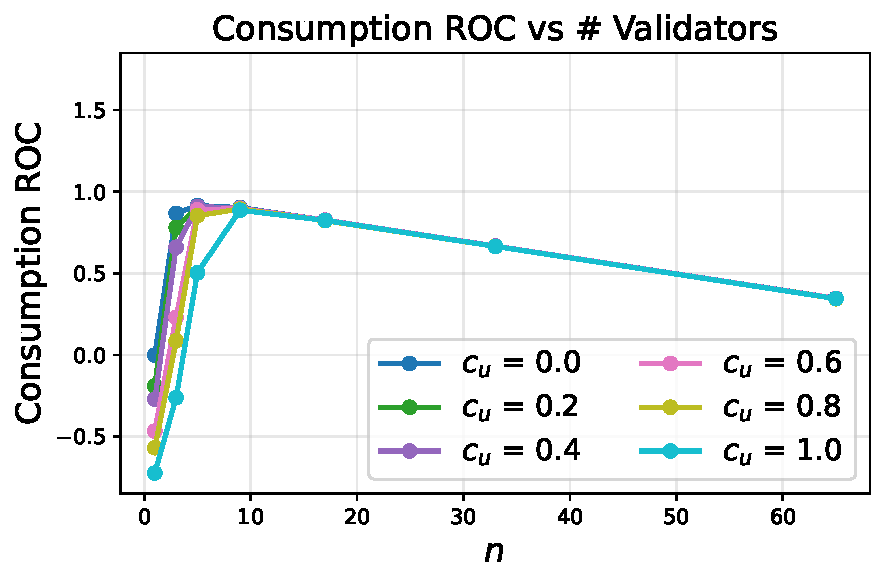
\includegraphics[width=\linewidth]{figures/hard/consumer_roc_all_costs.pdf}
        \caption{Consumption ROC}
    \end{subfigure}
    \hfill
    \begin{subfigure}[b]{0.195\linewidth}
        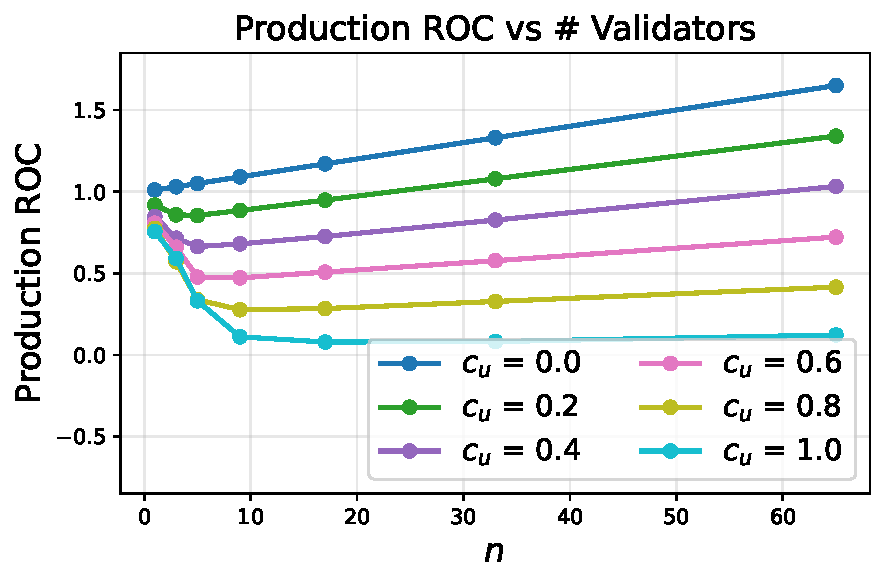
\includegraphics[width=\linewidth]{figures/hard/validator_roc_all_costs.pdf}
        \caption{Production ROC}
    \end{subfigure}
    \hfill
    \begin{subfigure}[b]{0.195\linewidth}
        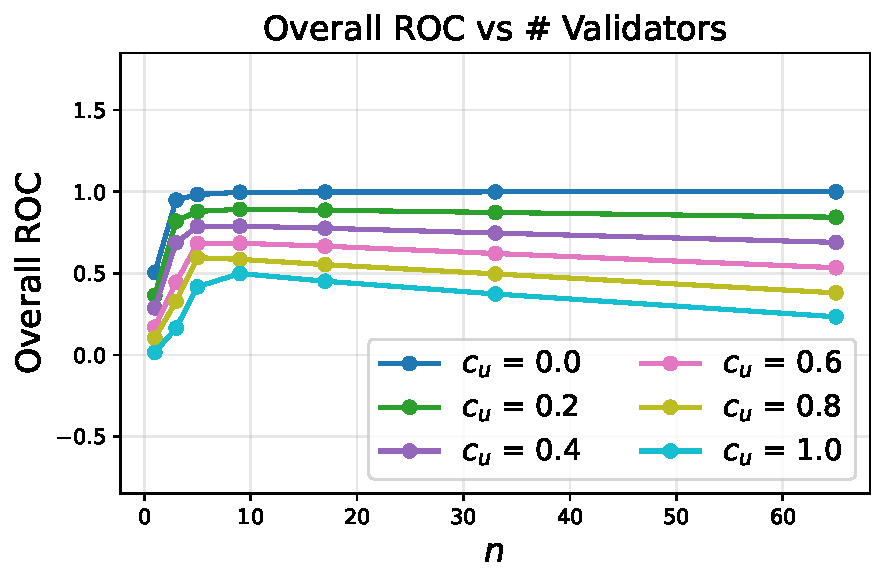
\includegraphics[width=\linewidth]{figures/hard/total_roc_all_costs.pdf}
        \caption{Overall ROC}
    \end{subfigure}
    \vspace{-2mm}
    \caption{Performance under different effort costs and validator counts. Larger committees improve posterior quality and consumer welfare up to a point, after which diminishing returns from increased validation cost reduce total welfare.}
    \label{fig:cost_validators}
    \vspace{0mm}
\end{figure*}

\begin{figure*}[t]
    \centering
    \begin{subfigure}[b]{0.15\linewidth}
        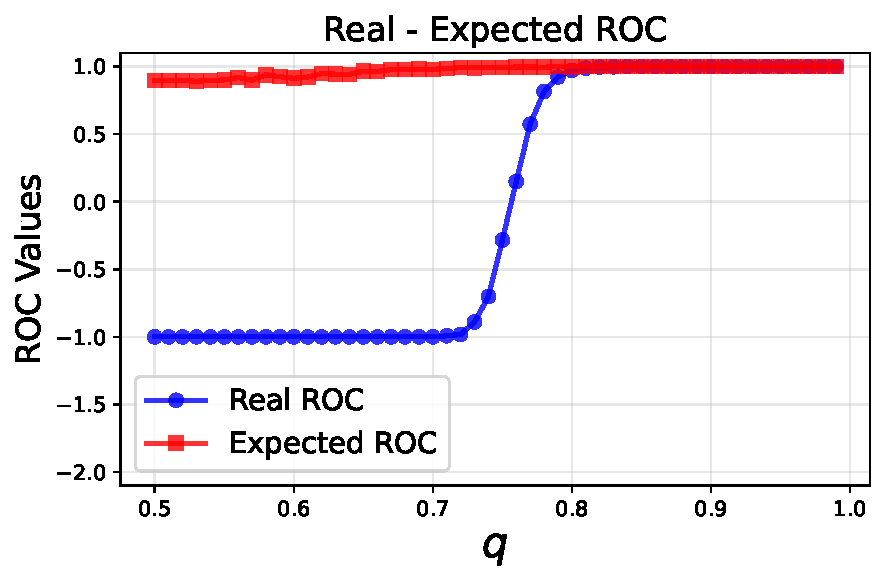
\includegraphics[width=\linewidth]{figures/quality/real_expected_roc_vs_p.pdf}
        \caption{Real ROC - \\Expected ROC}
    \end{subfigure}
    \begin{subfigure}[b]{0.15\linewidth}
        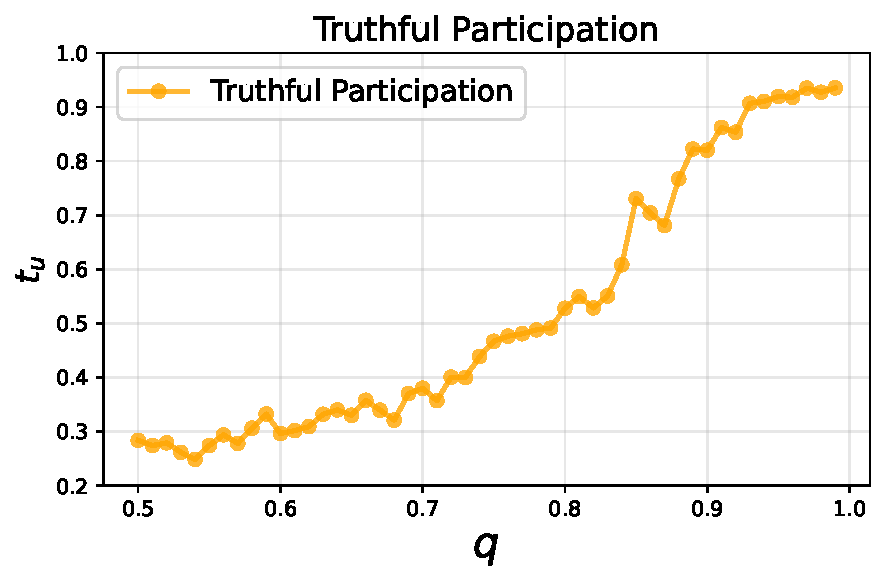
\includegraphics[width=\linewidth]{figures/quality/truthful_participation_vs_p.pdf}
        \caption{\textbf{\footnotesize Truthful \\Participation}}
    \end{subfigure}
    \begin{subfigure}[b]{0.15\linewidth}
        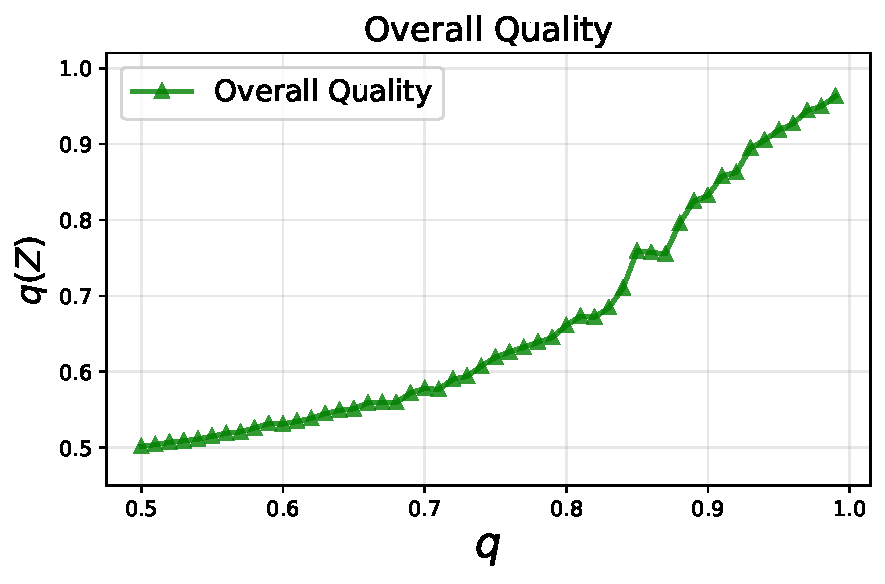
\includegraphics[width=\linewidth]{figures/quality/posterior_quality_vs_p.pdf}
        \caption{Overall \\Quality}
    \end{subfigure}
    \begin{subfigure}[b]{0.15\linewidth}
        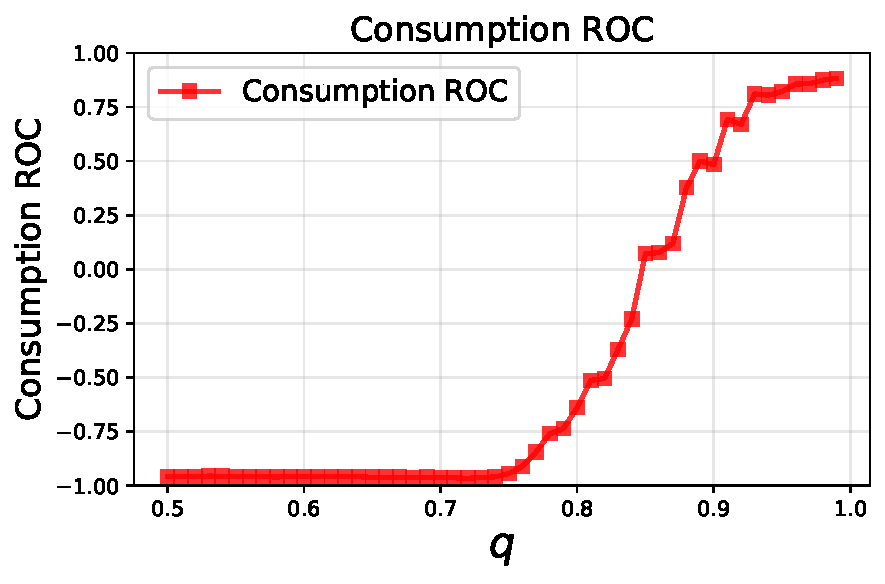
\includegraphics[width=\linewidth]{figures/quality/consumption_roc_vs_p.pdf}
        \caption{Consumption \\ROC}
    \end{subfigure}
    \begin{subfigure}[b]{0.15\linewidth}
        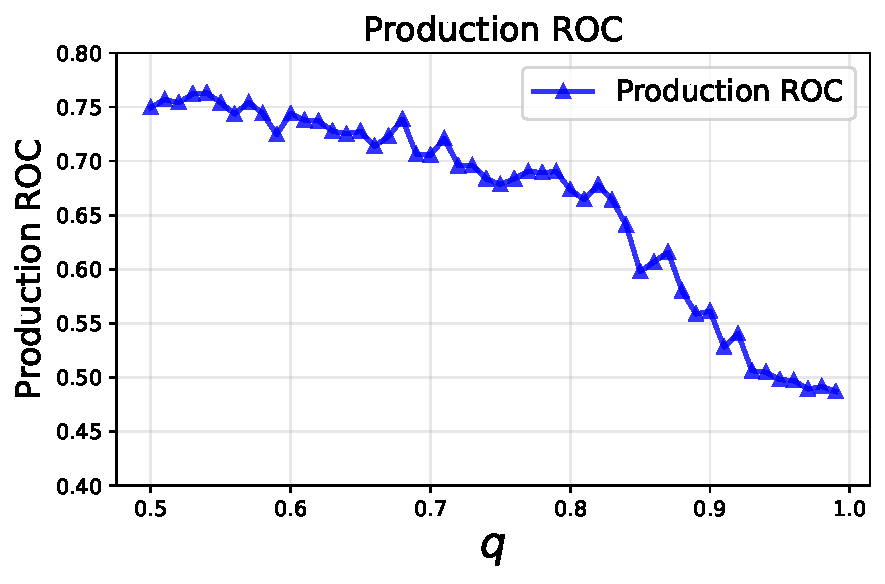
\includegraphics[width=\linewidth]{figures/quality/production_roc_vs_p.pdf}
        \caption{Production \\ROC}
    \end{subfigure}
    \begin{subfigure}[b]{0.15\linewidth}
        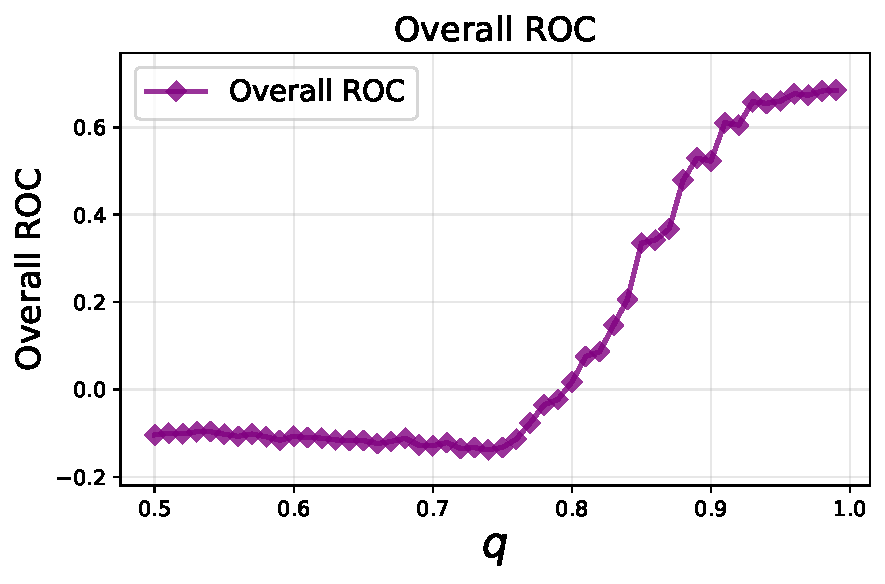
\includegraphics[width=\linewidth]{figures/quality/total_roc_vs_p.pdf}
        \caption{Overall \\ROC}
    \end{subfigure}
    \vspace{-2mm}
    \caption{Performance under different service quality levels. When producer quality is low ($q \approx 0.5$), the incentive mechanism cannot compensate, and welfare collapses. As quality increases, the mechanism amplifies honest effort into ecosystem-wide gains.}
    \label{fig:quality_impact}
\end{figure*}


\subsubsection{Instantiation}
In DeQA, the abstract ecosystem roles map to the QA domain as follows.
Consumer agents issue domain-specific \textit{queries} (e.g., medical, legal, scientific).
Producer agents provide \textit{answers} by invoking their knowledge-intensive service $a_u: \mathcal{Q} \rightarrow \mathcal{R}$, where $\mathcal{Q}$ is the query space and $\mathcal{R}$ the answer space.
Validator agents independently generate answers to the same queries and compare them against the producer's output, voting on agreement/disagreement to form the PoI consensus.
Service quality $q$ denotes the probability of generating a correct answer for a given query.


\subsubsection{Simulation Setting}

The simulation parameters are chosen to satisfy the theoretical assumptions while reflecting realistic operating conditions. We explain each choice and its connection to the formal model.

\textbf{(1) Agents and Roles.}
The system contains $N = 10{,}000$ agents, each randomly assuming the role of consumer, producer, or validator in each round.
Consumers issue queries uniformly across domains.
Agent service quality follows $q \sim 0.98 + 0.02\,\mathrm{Beta}(4,4) > \frac{1}{2}$, ensuring that Assumption~\ref{assum:validators} ($q_v > \frac{1}{2}$) is satisfied for all agents.
The Beta(4,4) distribution concentrates quality near the mean while allowing meaningful variance, modeling a population of generally competent but heterogeneous agents.
Agents selected randomly (without effort) have $q = \frac{1}{2}$, corresponding to the shirking case in Assumption~\ref{assum:binary}.
Each agent starts with $2{,}000$ tokens and exits once depleted, creating the finite-resource pressure that drives evolutionary dynamics.

\textbf{(2) Validation Mechanism.}
Validator count $n$ is odd (as required by Assumption~\ref{assum:validators}) and varied across $\{1, 5, 9, 17, 33, 65\}$ to test the comparative statics prediction that larger $n$ strengthens IC by raising $P_{\text{match}}$.
Each validation uses $m = 10$ sample queries, providing sufficient statistical power for consensus.
Validation fee $\tau_{\text{val}} = 1$ and stake $\sigma = 1$, satisfying $c_u < \tau_{\text{val}}$ (Assumption~\ref{assum:costs}) for all effort costs in our range.
Consensus is by majority vote, consistent with the theoretical model.
Each agent's strategy is parameterized by its truthful participation rate $t_u \in [0, 1]$ in both production and validation---when $t_u = 1$, the agent always exerts full effort ($e = 1$ in the formal model); when $t_u = 0$, it always shirks ($e = 0$).
Agents aim to maximize return on capital (ROC); low-ROC agents learn strategies from high-ROC agents, modeling the rational adaptive behavior predicted by the BNE dynamics.
Initial strategies are random ($t_u = \text{Uniform}(0, 1)$), representing a ``cold start'' ecosystem with no prior coordination.

\textbf{(3) Promotion and Subscription.}
Producers incur effort cost $c_u \in (0, 1)$ per validation query and receive $\tau_s = 1{,}000$ upon successful subscription.
The large ratio $\tau_s / \tau_{\text{val}} = 1{,}000$ ensures the cost ordering $mn\tau_{\text{val}} \ll \tau_s$ required by Assumption~\ref{assum:costs}, making validation economically viable relative to the subscription stakes.

\textbf{(4) System Assumptions and Simulation Protocol.}
Validators are independent and non-collusive (Assumption~\ref{assum:validators}). All parameters are finite and drawn from bounded intervals.
We simulate 100{,}000 \textit{interaction episodes}, where each episode constitutes one complete promotion--validation--subscription cycle: a consumer broadcasts a service need, a producer promotes, validators assess, and the consumer decides whether to subscribe.
Results are averaged over 5 independent random seeds; shaded regions in figures indicate $\pm 1$ standard deviation.

\textbf{(5) Evaluation Metrics.}
We evaluate three metrics, defined formally as follows:
\begin{itemize}
    \item \textbf{Truthful participation rate} $\bar{t} \coloneqq \frac{1}{|\mathcal{U}_{\text{active}}|} \sum_{u \in \mathcal{U}_{\text{active}}} t_u$, the population-averaged effort level.
    \item \textbf{Return on capital (ROC)}: for each agent $u$, $\text{ROC}_u \coloneqq (B_u^{\text{final}} - B_u^{\text{init}}) / B_u^{\text{init}}$, where $B_u^{\text{init}}$ and $B_u^{\text{final}}$ are the agent's initial and final token balances. Aggregate ROC is computed separately for consumers, producers, and the total population.
    \item \textbf{Social welfare} $W \coloneqq \sum_{u \in \mathcal{U}} \text{ROC}_u$, the sum of all agents' returns on capital, capturing the total economic surplus generated by the ecosystem. We also report consumer welfare $W_c$ and producer welfare $W_p$ to characterize surplus distribution.
    \item \textbf{Posterior quality} $\mathbb{E}[q_p \mid Z = 1]$, the expected producer quality conditional on passing validation, measuring the informativeness of the PoI mechanism.
\end{itemize}

\textbf{(6) Rationality Parameters.}
To study convergence \textit{toward} the BNE (rather than assuming agents start at equilibrium), we parameterize the population's rationality via two variables: $S_p \in [0, 1]$ denotes the proportion of agents that follow a rational learning rule (the remainder play fixed random strategies), and $S_u \in [0, 1]$ denotes the probability that a rational agent updates its strategy in a given round by imitating a higher-ROC peer. The case $S_p = S_u = 1$ corresponds to a fully adaptive population; $S_p = 0$ corresponds to a frozen, non-learning baseline.

\textbf{(7) Baselines.}
To contextualize our results, we compare against two natural baselines derived from the simulation itself:
\begin{itemize}
    \item \textbf{No-PoI} ($n = 0$): consumers subscribe based solely on the producer's self-reported performance declaration, without any third-party validation. This represents the information-asymmetry regime where the ``market for lemons'' operates unchecked.
    \item \textbf{Single-Validator} ($n = 1$): a single validator assesses service quality. As our IC analysis predicts (Theorem~\ref{Strict IC for Validators}), the lone validator faces minimal competitive pressure and is prone to shirking, since $P_{\text{match}} = q_v$ offers only a marginal advantage over random voting.
\end{itemize}
These baselines are not separate experiments but correspond to the boundary cases of our parameterized simulation, allowing direct comparison within the same experimental framework.

\subsubsection{Agent Rationality and Community Evolution (RQ1)}

We examine how the rationality parameters $S_p$ (proportion of adaptive agents) and $S_u$ (strategy update probability) influence ecosystem dynamics.

As shown in Figure~\ref{fig:roc_comp}, when agents never update strategies ($S_u = 1$, $S_p = 0$), producer surplus exceeds consumer surplus, but overall welfare remains low.
This baseline represents a ``frozen'' ecosystem where no learning occurs---producers who happen to shirk continue shirking, and consumers bear the cost of unreliable services.

When rational producers begin adapting by increasing $t_u$ (Figures~\ref{fig:roc_comp} and~\ref{fig:truthful_participation}), a striking pattern emerges:
individual producer surplus \textit{decreases} (higher effort means higher cost), but consumer surplus and total social welfare \textit{increase substantially}.
Low-ROC agents observe the success of high-$t_u$ agents and imitate their strategies, creating a population-level convergence toward honest participation.

\textbf{Theoretical connection.}
This result empirically confirms the tokenomics--knowledge dual loop: the incentive mechanism channels rational self-interest into collective welfare improvement.
Producers invest in truthful effort not out of altruism but because the mechanism makes honesty the utility-maximizing strategy---precisely the IC condition of Theorem~\ref{Strict IC for Validators} and the self-screening of Theorem~\ref{IR for Producers} in action.
The ecosystem acts as an evolutionary engine: agents that invest in quality thrive, while those that shirk are outcompeted and gradually exit.


\subsubsection{Validation Mechanism Analysis (RQ2)}

We analyze how committee size $n$ affects truthful participation, posterior quality, and welfare distribution.

\textbf{The monopoly problem ($n = 1$).}
As shown in Figure~\ref{fig:cost_validators}(a), with a single validator, the IC condition is barely satisfied: $P_{\text{match}} = q_v$ offers only a marginal advantage over random voting, and the sole validator can directly determine the consensus.
The result is pervasive shirking, low posterior quality, and consumer welfare losses.

\textbf{The benefits of competition ($n \uparrow$).}
As $n$ increases, mutual supervision emerges: each validator knows that deviating from the majority risks stake forfeiture, because the remaining validators are likely to produce a correct consensus.
Truthful participation becomes the dominant strategy (Figure~\ref{fig:cost_validators}(b)), and posterior quality improves significantly---validating the comparative statics prediction that larger $n$ expands the IC region.

\textbf{The cost trade-off.}
Although validation quality improves monotonically with $n$, the total cost $mn\tau_{\text{val}}$ also increases linearly.
Consumer benefits exhibit diminishing marginal returns (each additional validator adds less incremental information), while costs grow linearly.
The result is a welfare-optimal committee size: social welfare and consumer surplus first increase then decline with $n$ (Figures~\ref{fig:cost_validators}(c)(e)), while producer surplus exhibits the inverse pattern (Figure~\ref{fig:cost_validators}(d)).
In our setting, moderate committee sizes $n \in \{5, 9, 17\}$ achieve the best trade-off.


\subsubsection{Service Quality Impacts (RQ3)}

Finally, we investigate the fundamental relationship between producer knowledge quality and ecosystem welfare.

As shown in Figure~\ref{fig:quality_impact}(a), when producer quality is uniformly low, validation outcomes deviate substantially from truth.
Consumers make subscription decisions based on incorrect signals and suffer welfare losses.
In the extreme case $q = 0.5$, producers are no better than random---they cannot earn higher incentives through reliable service and become increasingly idle (Figure~\ref{fig:quality_impact}(b)).
Both consumer surplus and overall welfare turn negative (Figures~\ref{fig:quality_impact}(d)(e)(f)), reflecting a collapsed market.

As $q$ increases, a qualitative transition occurs: producer effort begins receiving positive feedback from the mechanism.
Higher quality $\Rightarrow$ higher pass probability $V_p(q_p)$ $\Rightarrow$ higher subscription revenue $\Rightarrow$ stronger incentive to maintain quality.
This positive feedback loop stabilizes the incentive environment, driving consumer surplus and total welfare into sustained growth (Figures~\ref{fig:quality_impact}(c)(e)(f)).

\textbf{Core insight.}
This result illuminates a fundamental design principle: \textit{our ecosystem is designed to reveal and reward existing capability, not to create it from nothing.}
When agents possess genuine domain knowledge, the tokenomics mechanism amplifies honest effort into ecosystem-wide gains.
When the knowledge base is fundamentally unreliable ($q \approx 0.5$), no incentive mechanism can compensate---the ecosystem degrades regardless of the economic design.
This underscores the complementary nature of the ecosystem and the underlying agent capabilities: the mechanism provides the right incentives, but the agents must bring genuine knowledge to the table.
